\documentclass[11pt]{article}

\usepackage{deauthor,times,graphicx}
% \usepackage[a4paper, total={6.7in, 9.7in}]{geometry}

% JobGraph fig
\usepackage{tikz}
\usetikzlibrary{arrows,automata,positioning,shapes.geometric}

% trademark symbol
\usepackage{textcomp}

\usepackage{float}

% code listings
\usepackage{listings}

\graphicspath{{submissions/submission4/figs/}}

\newcommand{\TODO}[1]{\textcolor{red}{TODO: #1}}
\newcommand{\sectionautorefname}{Section}%
\newcommand{\para}[1]{\vspace{2mm}\noindent\textbf{#1}}

\definecolor{dkgreen}{rgb}{0,0.6,0}
\definecolor{gray}{rgb}{0.5,0.5,0.5}
\definecolor{mauve}{rgb}{0.58,0,0.82}

% there is no built in support or Scala yet, good enough
\lstset{frame=l,
	language=Java,
	aboveskip=3mm,
	belowskip=3mm,
	showstringspaces=false,
	xleftmargin=5pt,
	%   framexleftmargin=-1pt,
	columns=flexible,
	basicstyle={\scriptsize\ttfamily},
	numbers=none,
	numberstyle=\tiny\color{black},
	keywordstyle=\color{blue},
	commentstyle=\color{dkgreen},
	stringstyle=\color{mauve},
	breaklines=true,
	breakatwhitespace=true,
	tabsize=4,
	%for scala
	emph={%
		object, def, val, zip, window, trigger, evict%
	},emphstyle={\color{blue}\textbf}%
}%


% \usepackage[
% % backend=biber
% % style=alphabetic,
% % sorting=abbrv
% ]{biblatex}

% \renewbibmacro{in:}{}


% \addbibresource{references.bib}
% \renewcommand{\bibfont}{\small} % or any other  appropriate font command

% url references
\usepackage{hyperref}

% in paragraph enums
\usepackage{paralist}

\usepackage{subfig}

\def\definitionautorefname{Definition}
\def\sectionautorefname{Section}
\def\subsectionautorefname{Section}
\def\subsubsectionautorefname{Section}
\def\algorithmautorefname{Algorithm}
\def\figureautorefname{Figure}

\usepackage{amsmath}
\usepackage{amsfonts}
\usepackage{booktabs}
\usepackage{amssymb}
\usepackage{dsfont}

\usepackage{multirow}

\usepackage{tablefootnote}

\usepackage{natbib}

\usepackage{lipsum}

\newcommand\blfootnote[1]{%
	\begingroup
	\renewcommand\thefootnote{}\footnote{#1}%
	\addtocounter{footnote}{-1}%
	\endgroup
}



\begin{document}

% Use the commands below, not some other ones.

\title{Differential Privacy for Time Series: A Survey}

\author{Yulian Mao\textsuperscript{1,2}, Qingqing Ye\textsuperscript{2 *}, Qi Wang\textsuperscript{1,3}, Haibo Hu\textsuperscript{2}\\
	\textsuperscript{1}\small{Department of Computer Science and  Engineering, Southern University of Science and Technology, Shenzhen, China}\\
	\textsuperscript{2}\small{Department of Electrical and Electronic Engineering, The Hong Kong Polytechnic University, Hong Kong SAR, China}\\
	\textsuperscript{3}\small{Shenzhen Key Laboratory of Safety and Security for Next Generation of Industrial Internet,  Shenzhen, China}\\
	\small{yulian.mao@connect.polyu.hk, qqing.ye@polyu.edu.hk, wangqi@sustech.edu.cn, haibo.hu@polyu.edu.hk}
}

\maketitle

\begin{abstract}
Time series are extensively used in finance, healthcare, IoT, and smart cities. However, in many applications, time series often contain personal information, so releasing them publicly can pose privacy risks. Differential privacy has recently emerged as the state-of-the-art approach for safeguarding data privacy. Unfortunately, adapting differential privacy to time series presents unique challenges compared to other data types due to their large volume, temporal correlations, and dynamic nature. To address users' demands for time series analysis while simultaneously protecting privacy, a significant body of research works have been proposed. The aim of this survey is to summarize these works and provide a holistic view of the DP mechanisms under differential privacy. Furthermore, we will discuss the challenges associated with time series release, especially in one of its most prevalent applications --- location based services. Finally, we will explore open challenges and shed light on directions for future research.


\end{abstract}

% Body of paper.  The paper should be present as a single file.
% Do not include other files for sections of the paper.
% Papers should not be longer than 12 pages

% ALL FIGURES MUST BE IN A SUBFOLDER NAMED figs
% See fig-guide for advice about figures
% Your paper's pdf should be less than 500K bytes

% Figures should be include in your paper using
% the \includegraphics command


\vspace{-1em}
\blfootnote{* Dr. Qingqing Ye is the corresponding author.}
% YOUR PAPER GOES HERE
\section{Introduction}
Time series are being generated on a large scale across a wide range of application domains, such as IoT, finance, healthcare monitoring, operational event logs, and smart home sensors. For example, smart home devices such as thermostats and humidity sensors generate continuous time series on environmental conditions, tracking temperature fluctuations and moisture levels to optimize home climate control based on user activities. Additionally, trajectories represent a unique type of time series that contain both spatial and temporal information, such as GPS data tracking the movement of vehicles or individuals. To facilitate the analysis of time series and support various downstream tasks,  numerous methods have been proposed, ranging from traditional statistical techniques, such as ARIMA~\cite{hyndman2018forecasting} and exponential smoothing~\cite{gardner2006exponential}, to advanced machine learning models, such as long short-term memory (LSTM) networks~\cite{shi2015convolutional}. However, a key issue in these time series applications is privacy. Since many data sources such as smart home sensors and location trajectories contain individuals' private information, the direct release or analysis of such time series can lead to significant privacy violations. Consequently, developing privacy-preserving mechanisms for time series analysis is essential.

Differential privacy (DP) ~\cite{Dwork2006} is a paradigm of privacy-preserving mechanisms that provides a theoretical privacy guarantee and has been further extended to the local setting to accommodate more general scenarios~\cite{ye2020local, Yang2023}. Numerous DP mechanisms have been developed to support various queries~\cite{wang2017locally, wang2018privacy, wang2019locallyhv}, including estimating statistics such as frequency~\cite{wang2017locally, fu2023collecting} and mean~\cite{li2020estimating}, ensuring that the privacy of individuals in the dataset is protected even when aggregate information is released. Recently, research has shifted towards more complex applications, such as graph data mining~\cite{ye2020towards} and machine learning problems~\cite{zhang2012functional}. Techniques such as differentially private stochastic gradient descent (DP-SGD)~\cite{abadi2016deep, fu2023dpsur} have been developed to train machine learning models with differential privacy guarantees, enabling the use of private datasets for tasks like classification and prediction without compromising individuals' privacy. It is worth noting that differential privacy is also being explored in the context of time series~\cite{dwork2010differential, chan2011private, Kellaris14}. This involves developing new mechanisms capable of handling the features of time series, ensuring that privacy is maintained.

Nevertheless, time series data present more challenges compared to other types of data due to their large volume, temporal correlation, and dynamic nature. The large volume, in particular, poses significant issues for privacy models, as protecting every element of a time series would degrade utility. To address this challenge, three privacy levels have been proposed~\cite{Kellaris14}: event-level privacy, which protects a single element in the time series; $w$-event level privacy, which provides a privacy guarantee for $w$ consecutive elements; and user-level privacy, which protects all elements associated with an individual. To enhance utility, sampling and filtering-based mechanisms~\cite{fan2013adaptive}, as well as privacy budget allocation strategies~\cite{Kellaris14}, have been suggested. Additionally, the correlations between elements can lead to privacy breaches~\cite{shao2020structured}, necessitating countermeasures to confine these correlations~\cite{cao2017quantifying, xiao2017loclok}. Given numerous research efforts in this field,  a taxonomy is necessary to summarize the existing works and identify areas for future research.

However, to the best of our knowledge, there is no up-to-date and comprehensive survey specifically for time series under differential privacy. Dwork and Roth~\cite{dwork2014algorithmic} coauthored a comprehensive survey on differential privacy, which seems outdated now in terms of state-of-the-art techniques. More recently, there are two surveys from Zhao et al.~\cite{zhao2022survey, zhao2024scenario} focusing on the concepts and applications of differential privacy, but they do not extensively cover time series.
Miranda-Pascual et al.~\cite{miranda2023sok} conducted a survey on trajectory data publication, which mainly talks about downstream tasks with little emphasis on privacy preservation. %In contrast, our literature review on trajectories is based on emergent privacy issues and the demand for trajectory release. 
The most relevant survey on time series under differential privacy is by Katsomallos et al.~\cite{katsomallos2019privacy}. However, since it was published in 2019, the paper does not reflect current technical trends, such as LDP, which now accounts for a crucial portion of privacy-preserving time series research. %Therefore, we present this survey to review time series under differential privacy and suggest future research directions.


%In this survey, we aim to provide a brief introduction to time series under differential privacy. Since the sequential nature of time series, it has three distinct privacy levels, each offering different degrees of privacy guarantees. Additionally, the complexity of basic queries in time series analysis necessitates a detailed introduction. We start by discussing the count query, which extends to more advanced estimations like frequency and histograms. Following this, we delve into sum and mean queries, including range queries of the sum. Furthermore, we examine various works focused on time series release. This part is categorized based on the type of content released: either through value perturbation or through the generation of synthetic data. We also emphasize a specific and popular application of time series: location-based services. In this context, we review papers according to their privacy models and the downstream applications they support. In our discussion of future directions, we highlight four key challenges according to privacy models, potential attacks, data types, and learning problems.

% describe the difficulty

In this survey, we aim to provide a comprehensive review of research works on time series under differential privacy. The main contents and paper organization are summarized as follows.
\begin{itemize}
	\item \textbf{Section~\ref{sec2}: Fundamental concepts of time series and differential privacy.} We first introduce the basic concepts of time series and differential privacy, including the definitions of differential privacy and the composition theorems. Additionally, we elucidate the three privacy levels specifically defined within the context of time series.
	\item \textbf{Section~\ref{sec3}: Count queries and corresponding advanced queries.} We begin with an introduction to count queries, and then present two core techniques for their realization: the binary tree-based mechanism~\cite{chan2011private} and the matrix mechanism~\cite{li2015matrix}. Following this, we discuss advanced queries, such as frequency and histogram estimations, which are based on count queries. Finally, we explore downstream applications derived from count queries.
	\item \textbf{Section~\ref{sec4}: Sum/mean queries and downstream applications.} We list sum and mean queries together  due to their inherent correlation. Following the introduction of sum and mean queries, we present the developed mechanisms for these queries. Subsequently, we review the literature on downstream applications.
	\item \textbf{Section~\ref{sec5}: Time series release.} We classify the literature into two categories: methods based on value perturbation and  methods based on synthesis. For value perturbation-based methods, we first review  privacy budget allocation strategies and then present the optimization strategies to improve utility. We then  introduce the synthesis-based methods, including those based on statistics and generative models. Additionally, we discuss the privacy models of the time series mechanisms and review a line of work that perturbs the temporal order rather than the values to accommodate value-critical scenarios.
	\item \textbf{Section~\ref{sec6}: Location based services and trajectory release.} Given that location based services are common applications under differential privacy, we dedicate a section to discussing the relevant literature.  To improve the utility, geo-indistinguishability~\cite{andres2013geo} was proposed to constrain the perturbation domain. Moreover, due to the apparent temporal correlation, the relationships between locations need to be considered. Finally, we present mechanisms designed for trajectory release based on perturbation and synthesis.
    \item \textbf{Section~\ref{sec7}: Open challenges.} We present a few future research directions for DP-based time series in terms of privacy model, potential correlation-based attacks, complex data type, and learning based problems.
\end{itemize}



%The remainder of this paper is organized as follows. Section~\ref{sec2} introduces the preliminaries on time series and differential privacy. Section~\ref{sec3} summarizes count queries under differential privacy, while Section~\ref{sec4} reviews sum and mean queries. Section~\ref{sec5} focuses on the time series release problem. Section~\ref{sec6} discusses mechanisms related to location based services. Finally, Section~\ref{sec7}  proposes some open challenges and Section 8 concludes the survey.


\section{Preliminaries}\label{sec2}
In this section, we first introduce the basic concepts of differential privacy and differential privacy for time series. As for the latter, we mainly focus on different privacy levels of DP mechanisms used to analyze time series.

\subsection{Differential Privacy}
% differential privacy
Differential privacy is a rigorous and practical formalization that provides a quantitative measure of privacy leakage for an individual when participating in a database~\cite{Dwork2006}. In the nearly 20 years since its inception, differential privacy has become widely adopted as a privacy-preserving framework. Many companies, such as Microsoft~\cite{Ding2017}, Google~\cite{Erlingsson2014}, and Apple~\cite{Thakurta2017}, utilize differential privacy to collect users' data while providing privacy guarantees.  Additionally, the US Census Bureau adopted differential privacy for the 2020 decennial census~\cite{Dwork2019}.

Based on utilization scenarios, differential privacy can be broadly categorized into centralized differential privacy (CDP) and local differential privacy (LDP)~\cite{Yang2023}. Centralized differential privacy requires a trusted third party to act as the data curator, collecting data from users and releasing the processed results to the public. The trusted third party is assumed to safeguard private information and not disclose it. However, in many situations, such a trusted third party may not exist.  Consequently, local differential privacy has been proposed, allowing data to be sanitized locally before being uploaded. These two different  scenarios are depicted in Fig~\ref{cdp-ldp}, and their formal definitions are provided below.

\begin{figure}[htbp]
	\centering
		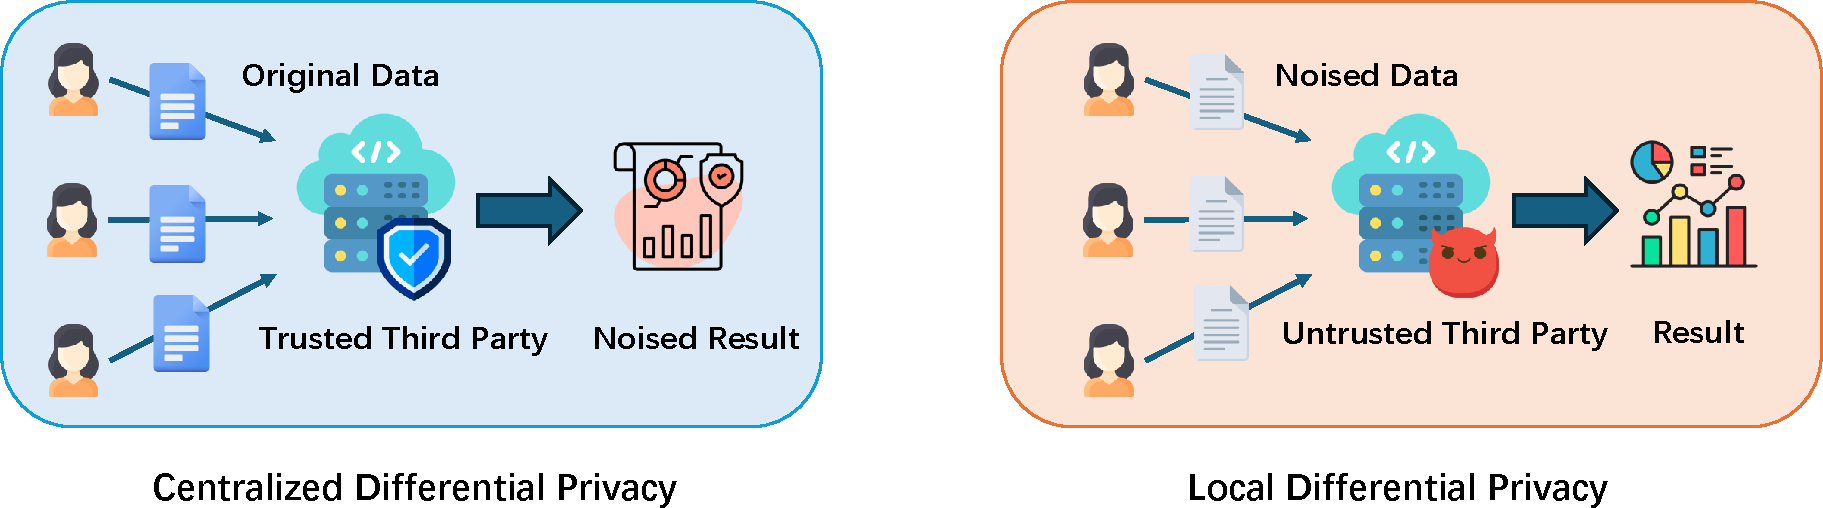
\includegraphics[width=0.7\textwidth]{submissions/submission4/figs/02-pre/cdp-ldp-crop.pdf}
	\caption{An illustration for centralized differential privacy and local differential privacy. In the context of centralized differential privacy, a trusted third party collects original data from users and adds noise to the processed result. In contrast, under  local differential privacy, users add noise to their data locally before uploading the noised data to the untrusted third party.}
	\label{cdp-ldp}
\end{figure}

\subsubsection{Centralized Differential Privacy (CDP)}
Before delving into the formal definition of centralized differential privacy, it is important to first elucidate some underlying concepts. We start with the definition of  neighboring datasets.
%Since CDP prevents distinguishing an individual from a group, datasets that differ by only one record from an individual are referred to as neighboring datasets~\cite{dwork2014algorithmic}.
\begin{definition}[Neighboring Datasets~\cite{dwork2014algorithmic, zhao2022survey, li2017differential}]
	Two datasets $D$ and $D'$ are \textit{neighboring} if they only differ by only one record. In \textit{Unbounded CDP}, $D$ can be obtained from $D'$ by adding or removing one record, whereas in \textit{Bounded DP}, $D$ can be obtained from $D'$ by replacing one record.
\end{definition}

\begin{definition}[$(\epsilon, \delta)$-Centralized Differential Privacy ($(\epsilon, \delta)$-CDP)~\cite{dwork2014algorithmic, zhao2022survey, li2017differential}] A randomized mechanism $\mathcal{M}$ satisfies $(\epsilon, \delta)$-centralized differential privacy if and only if for any two neighboring datasets $D$, $D'$, and any possible output $R\subseteq\mathrm{Range}(\mathcal{M})$, there is
	\begin{equation}
		\mathrm{Pr}[\mathcal{M}(D)=R]\le e^\epsilon\cdot \mathrm{Pr}[\mathcal{M}(D')=R]+\delta.\nonumber
	\end{equation}
When $\delta=0$, $\mathcal{M}$ satisfies $\epsilon$-centralized differential privacy.
\end{definition}



% local differentail privacy
\subsubsection{Local Differential Privacy (LDP)}
As we aforementioned, local differential privacy is adopted in a local mode. Compared with CDP, LDP requires more added noise to ensure privacy but does not need a trusted third party. Therefore, neighboring datasets in LDP can be any input from users.
\begin{definition}[$(\epsilon, \delta)$-local differential privacy ($(\epsilon, \delta)$-LDP)~\cite{zhao2022survey, li2017differential}]
A randomized mechanism $\mathcal{A}$ satisfies $(\epsilon, \delta)$-local differential privacy if and only if for any inputs $v$, $v'$, and any possible output $r\subseteq\mathrm{Range}(\mathcal{A})$, there is
\begin{equation}
	\mathrm{Pr}[\mathcal{A}(v)=r]\le e^\epsilon\cdot \mathrm{Pr}[\mathcal{A}(v')=r]+\delta.\nonumber
\end{equation}
When $\delta=0$, $\mathcal{A}$ satisfies $\epsilon$-local differential privacy which is also called pure-LDP~\cite{wang2017locally}.
\end{definition}

\subsubsection{Composition Theorems}
Under differential privacy (both CDP and LDP), there are two useful composition theorems~\cite{li2017differential}: sequential composition and parallel composition.

\begin{definition}[Sequential Composition~\cite{li2017differential}]
	Given a dataset $x$, and two mechanisms $M_1$, $M_2$ satisfy $(\epsilon_1, \delta_1)$-DP and $(\epsilon_2, \delta_2)$-DP, respectively, the mechanism $M=(M_1(x), M_2(x))$ satisfies $(\epsilon_1+\epsilon_2, \delta_1+\delta_2)$-DP.
\end{definition}

\begin{definition}[Parallel Composition~\cite{li2017differential}]
	Given a mechanism $M$ satisfy $(\epsilon, \delta)$-DP, and the $k$ disjoint separations of the dataset $x$ (i.e., $x_1\cup x_2\cup \cdots \cup x_k=x$), the release $M(x_1), M(x_2), \cdots, M(x_k)$ satisfies $(\epsilon, \delta)$-DP.
\end{definition}

% sequential composition


% parallel composition

\subsubsection{Pufferfish Privacy}
When providing privacy guarantees for correlated time series, differential privacy faces the challenge of excessive noise addition. Specifically, group differential privacy~\cite{dwork2014algorithmic} necessitates adding $O(T)$ noise for a  correlated time series with length $T$, leading to significant utility degradation. To address correlated data, pufferfish privacy, a generalized version of differential privacy, was proposed~\cite{kifer2014pufferfish}. In addition to the privacy budget $\epsilon$, pufferfish privacy requires three additional parameters~\cite{song2017pufferfish}: a set of secrets $\mathcal{S}$ representing users' private data, a set of secret pairs $\mathcal{Q}\subseteq \mathcal{S}\times \mathcal{S}$ that must remain indistinguishable, and a class of data distribution $\Theta$ indicating the correlation.
\begin{definition}[$\epsilon$-Pufferfish Privacy~\cite{song2017pufferfish}]
Give the parameters $\mathcal{S}$, $\mathcal{Q}$, and $\Theta$, a randomized mechanism $M$ satisfies $\epsilon$-pufferfish privacy if $\forall \theta\in \Theta $ with $X\sim \theta$, $\forall (s_i, s_j)\in \mathcal{Q}$, $\forall w\in \text{Range}(M)$, there is
\begin{equation}\nonumber
 \mathrm{Pr}(M(X)=w|s_i, \theta)\le e^\epsilon\cdot \mathrm{Pr}(M(X)=w|s_j, \theta),
\end{equation}
when $\mathrm{Pr[s_i|\theta]\ne 0}$ and $\mathrm{Pr[s_j|\theta]\ne 0}$.
\end{definition}
%For more detailed information about pufferfish privacy, readers are recommended to refer to~\cite{kifer2014pufferfish, song2017pufferfish}.





\subsubsection{Differential Privacy Mechanisms}
Given that noise addition from a distribution is a fundamental implementation of differential privacy, this technique is extensively used for statistical estimation. Numerous applications rely on count queries, including frequency estimation, histogram estimation, and top-$k$ item mining. Korolova et al. \cite{korolova2009releasing} introduced a mechanism for releasing search log histograms by adding Laplace noise. Xiao et al. \cite{xiao2010differential} proposed a wavelet-based mechanism to release range count queries. In the context of LDP, Wang et al. \cite{wang2017locally} reviewed existing mechanisms for frequency estimation and introduced two optimized approaches. Li et al. \cite{li2020estimating} developed a mechanism for estimating numerical data distributions. Wang et al. \cite{wang2019locallyhv} proposed a prefix extension mechanism to identify the top-$k$ frequent items within a large domain. Beyond count queries, many applications focus on sum or mean queries. Wang et al. \cite{wang2019collecting} devised a mechanism with optimized perturbation probability for numerical data under LDP. Xue et al. \cite{xue2022mean} introduced a mean estimation mechanism that supports personalized privacy budgets for each user. Zhou et al. \cite{zhou2022locally} developed a mechanism to estimate the mean of sparse vectors. To incorporate data knowledge, Wei et al. \cite{wei2024aaa} proposed an optimized mean estimation mechanism based on data distribution estimated in the initial phase under LDP. Beyond statistical estimations, data release for downstream tasks is another critical application. Ye et al. \cite{ye2020lf} proposed a mechanism to release edge information for clustering coefficient estimation. Ma et al. \cite{ma2024decision} developed a mechanism to construct decision trees under LDP, enhancing utility through the adoption of public data. Additionally, since the introduction of Differentially Private Stochastic Gradient Descent (DP-SGD) \cite{abadi2016deep}, numerous privacy-preserving learning-based mechanisms have been proposed under differential privacy.

Across the various scenarios, time series represent a unique research field due to their sequential nature and temporal dependencies. This adds complexity to ensuring differential privacy while maintaining data utility. In the following sections, we will introduce the concepts of time series under differential privacy.



\subsection{Differential Privacy for Time Series}
In this subsection, we will introduce the concept of time series and the specific definitions of differential privacy for time series, including various privacy levels. Additionally, we will provide a concise roadmap of this survey.

\subsubsection{Time Series}
In general, a time series is regarded an ordered sequence of values with finite length~\cite{esling2012time}, while data streams are continuously generated sequences with infinite length~\cite{silva2013data}. For ease of presentation, both are referred to as ``time series" in this paper, encompassing both finite and infinite settings.

% offline
%\begin{definition}[Finite Time Series~\cite{esling2012time, ruiz2021great}] A finite time series $S$ is an ordered sequences of values with a fixed length, i.e., $S=\{S_{t_1}, S_{t_2}, S_{t_3}, \cdots, S_{t_n}\}$. For simplicity, the timestamp is usually omitted, and a time series is denoted as $S=\{S_{1}, S_{2}, S_{3}, \cdots, S_{n}\}$. If any element $S_i\in \mathbb{R}$, the time series is called a univariate finite time series. Otherwise, if $S_i\in \mathbb{R}^d$,  it is referred to as a multivariate finite time series, meaning each element has $d$ dimensions.
%	
%\end{definition}


% online
\begin{definition}[Time Series~\cite{esling2012time, silva2013data, ruiz2021great}] A time series $S$ is an ordered sequences of values, i.e., $S=\{S_{t_1}, S_{t_2}, S_{t_3}, \cdots\}$. For simplicity, the timestamp is usually omitted, and a time series is denoted as $S=\{S_{1}, S_{2}, S_{3}, \cdots\}$. If any element $S_i\in \mathbb{R}$, the time series is called a univariate infinite time series. Otherwise, the time series is a multivariate infinite time series if $S_i\in \mathbb{R}^d$, namely, each element is with $d$ dimensions.
\end{definition}

Note that if a time series has a finite length, it is called a finite time series. Otherwise, it is referred to as an infinite time series.


\subsubsection{Privacy Levels}
In the context of time series, three major privacy levels have been proposed based on the privacy guarantees. Event-level privacy only protects a single element within a time series, $w$-event level privacy provides a privacy guarantee for a sequence of $w$ consecutive elements, and user-level privacy protects the entire time series. The corresponding definitions are provided below, with illustrations depicted in Fig.~\ref{privacy_level}.

\begin{definition}[Event-Level Adjacent Time Series~\cite{Kellaris14}]
	For two time series $S$ and $S'$, they are event-level adjacent if
	\begin{enumerate}
		\item [1)] There exists a timestamp $i$, $S_i\ne S'_i$;
		\item [2)] For any other timestamp $j$,  $S_j= S'_j.$
	\end{enumerate}
\end{definition}

\begin{definition}[Event-Level Privacy~\cite{Kellaris14}] A randomized mechanism $\mathcal{M}$ satisfies $(\epsilon, \delta)$-event-level differential privacy if and only if for any two event-level adjacent time series $S$, $S'$, and any possible output $R\subseteq\mathrm{Range}(\mathcal{M})$, there is
	\begin{equation}
		\mathrm{Pr}[\mathcal{M}(S)=R]\le e^\epsilon\cdot \mathrm{Pr}[\mathcal{M}(S')=R]+\delta.\nonumber
	\end{equation}
	When $\delta=0$, $\mathcal{M}$ satisfies $\epsilon$-event-level differential privacy.
\end{definition}

\begin{definition}[$w$-Event Level Adjacent Time Series~\cite{Kellaris14}]
	For two time series $S$ and $S'$, they are  $w$-event level adjacent if
	\begin{enumerate}
		\item [1)] There exists $w$ consecutive timestamp $\{k, k+1, \cdots, k+w-1\}$ and for any $i \in \{k, k+1, \cdots, k+w-1\}$, $S_i\ne S'_i$;
		\item [2)] For any other timestamp $j$,  $S_j= S'_j.$
	\end{enumerate}
\end{definition}

\begin{definition}[$w$-Event Level Privacy] A randomized mechanism $\mathcal{M}$ satisfies $(\epsilon, \delta)$-$w$-event level differential privacy if and only if for any two $w$-event level adjacent time series $S$, $S'$, and any possible output $R\subseteq\mathrm{Range}(\mathcal{M})$, there is
	\begin{equation}
		\mathrm{Pr}[\mathcal{M}(S)=R]\le e^\epsilon\cdot \mathrm{Pr}[\mathcal{M}(S')=R]+\delta.\nonumber
	\end{equation}
	When $\delta=0$, $\mathcal{M}$ satisfies $\epsilon$-$w$-event level differential privacy.
\end{definition}

\begin{definition}[User-Level Adjacent Time Series]
	For two time series $S$ and $S'$, they are user-level adjacent if for all timestamps $t_{u_i}=\{t_1, t_2, \cdots , t_k\}$  from any user $u_i$, there is $S_j\ne S'_j, \forall j\in t_{u_i}$. Note that $t_{u_i}$ can be infinite for infinite time series.
\end{definition}

\begin{definition}[User-Level Privacy] A randomized mechanism $\mathcal{M}$ satisfies $(\epsilon, \delta)$-user-level differential privacy if and only if for any two user-level adjacent time series $S$, $S'$, and any possible output $R\subseteq\mathrm{Range}(\mathcal{M})$, there is
	\begin{equation}
		\mathrm{Pr}[\mathcal{M}(S)=R]\le e^\epsilon\cdot \mathrm{Pr}[\mathcal{M}(S')=R]+\delta.\nonumber
	\end{equation}
	When $\delta=0$, $\mathcal{M}$ satisfies $\epsilon$-user-level differential privacy.
\end{definition}

\begin{figure}[H]
	\centering
	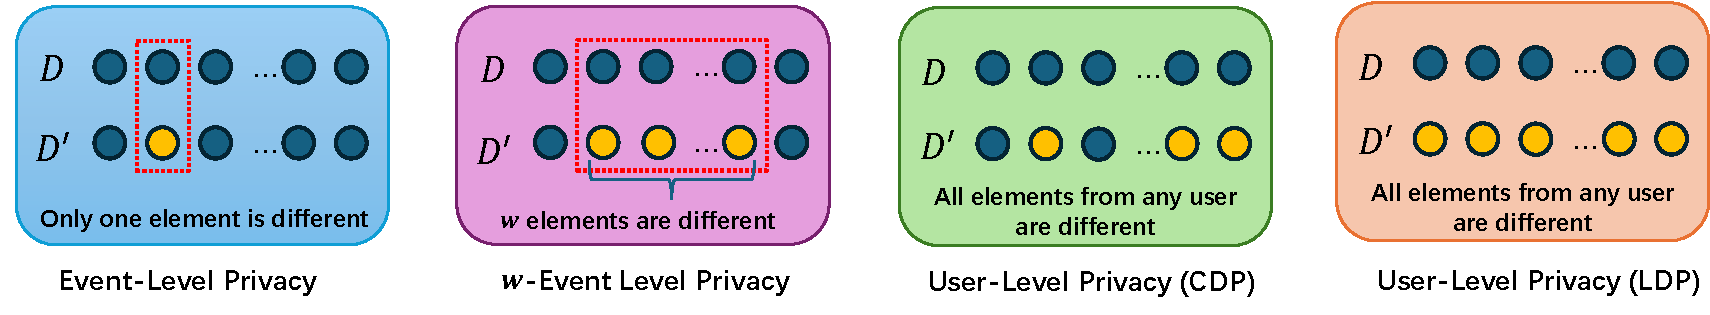
\includegraphics[width=0.8\textwidth]{submissions/submission4/figs/02-pre/privacy_level-crop.pdf}
	\caption{An illustration for privacy levels. In terms of event-level privacy, there is only one element different in the neighboring datasets. While for the $w$-event level privacy, there are $w$ consecutive elements that differ in the neighboring datasets. For user-level privacy, all the elements from any user can be different in the neighboring datasets. Note that under LDP, the two user-level adjacent time series are from different users, which means the elements could be entirely different. }
	\label{privacy_level}
\end{figure}


Obviously, event-level privacy provides the lowest level of privacy but requires the least amount of noise. Conversely, user-level privacy guarantees the strongest privacy but necessitates the largest amount of noise, which can significantly degrade utility.


\subsection{Roadmap of This Survey}
Since count queries and sum/mean queries are fundamental statistical operations, many advanced queries and downstream applications are derived from them. This survey begins with a review on count queries, followed by a discussion of sum/mean queries.  Each subsection on these queries starts with an introduction to the concepts, followed by a review of their downstream applications. Subsequently, we introduce data release mechanisms designed to publicize data for downstream tasks. Given the popularity of location based services in time series applications, we dedicate a separate section to trajectories, reviewing the literature on  location perturbation, temporal correlation issues, and trajectory release. To suggest future directions, we propose open challenges related to privacy models, temporal correlation-based attacks, complex data types, and learning-based problems. The roadmap for this survey is illustrated in Fig.~\ref{rm}.
\begin{figure}[htbp]
	\makebox[\textwidth][c]{%
	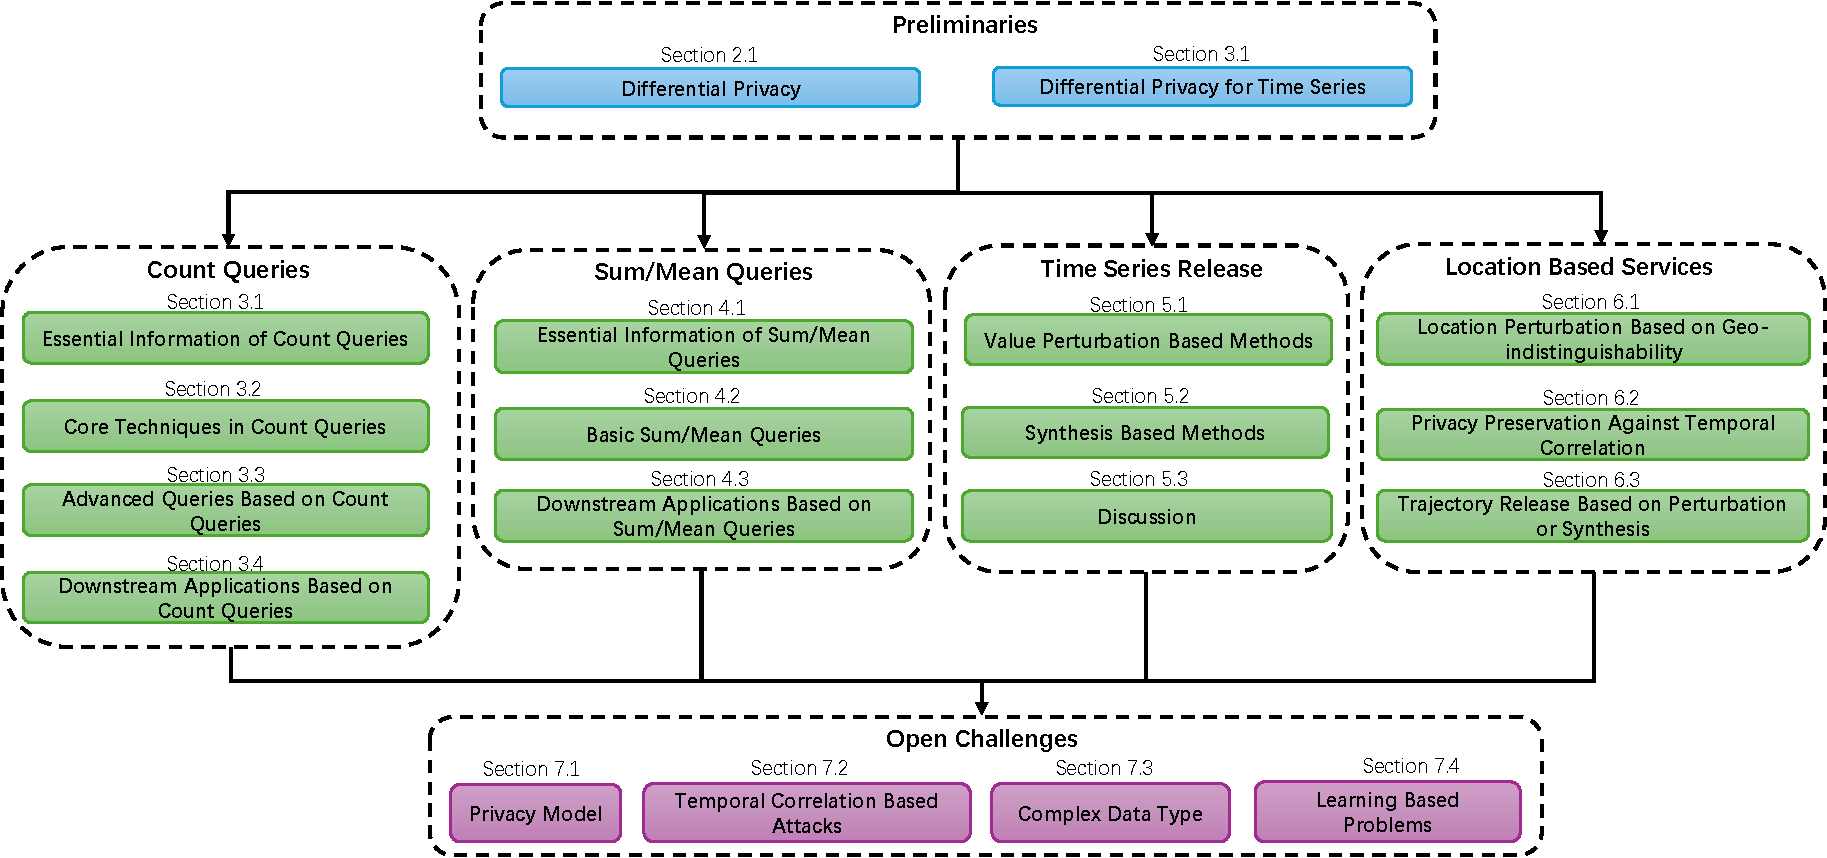
\includegraphics[width=1.1\textwidth]{submissions/submission4/figs/02-pre/roadmap-crop.pdf}
}
	\caption{Roadmap of this survey.}
	\label{rm}
\end{figure}









\section{Differential Privacy for Count Queries }\label{sec3}
In this section, we introduce the concept of count queries within the framework of differential privacy,  a topic that has garnered substantial research attention.

\subsection{Essential Information of Count Queries}
For a time series $S$ comprising categorical values with length $t$ ($t$ can be $\infty$), a count query can be formally expressed as follow:
\begin{equation}\nonumber
	\mathrm{F}_{\mathrm{cnt}}(v, S)=\sum_{i=1}^{t}\mathbf{1}_v(x_i),
\end{equation}
where $\mathbf{1}_v(x_i)$ denotes the indicator function, defined below:
\begin{equation}\nonumber
	\mathbf{1}_v(x_i) :=
	\begin{cases} 
		1 & \text{if } x_i=v, \\
		0 & \text{if } x_i \ne v.
	\end{cases}
\end{equation}
Count queries are fundamental in the context of differential privacy, as they form the basis for other tasks, such as frequency and histogram estimations. 
 Compared with other scenarios, applying count queries to time series presents unique challenges. Time series arrives as a continuous stream, necessitating the injection of a larger amount of noise to provide the desired privacy guarantees due to continuous release of query results. 
 


\subsection{Core Techniques in Count Queries}
For continuously releasing a finite time series, a naive approach is to release each element with the entire privacy budget $\epsilon$~\cite{chan2011private}. However, such a method would introduce substantial additive noise, leading to low utility with an error bound of $O(\frac{\sqrt{T}}{\epsilon})$. 
Dwork et al.~\cite{dwork2010differential} proposed the first work to handle binary time series under event-level CDP with a logarithm error bound. However, this mechanism is limited to time series with finite length $T$. Subsequently, Chan et al.~\cite{chan2011private} improved the mechanism to support the release of infinite binary time series. Both of these works employ a tree-based method to enhance utility. The binary tree mechanism~\cite{chan2011private}, illustrated in Fig.~\ref{tree_mechanism}, ensures that each release influences at most one node at each level for finite time series. Consequently, each node only needs to add noise corresponding to the privacy budget $\frac{\epsilon}{(\log T+1)}$. To guarantee a logarithm error bound for infinite time series~\cite{chan2011private, dong2023continual}, more binary trees will be construed. Since the update of one element only influences one tree, each tree will be allocated an entire privacy budget. More details can be referred to Fig.~\ref{tree_mechanism}.

\begin{figure}[h]
	\centering
	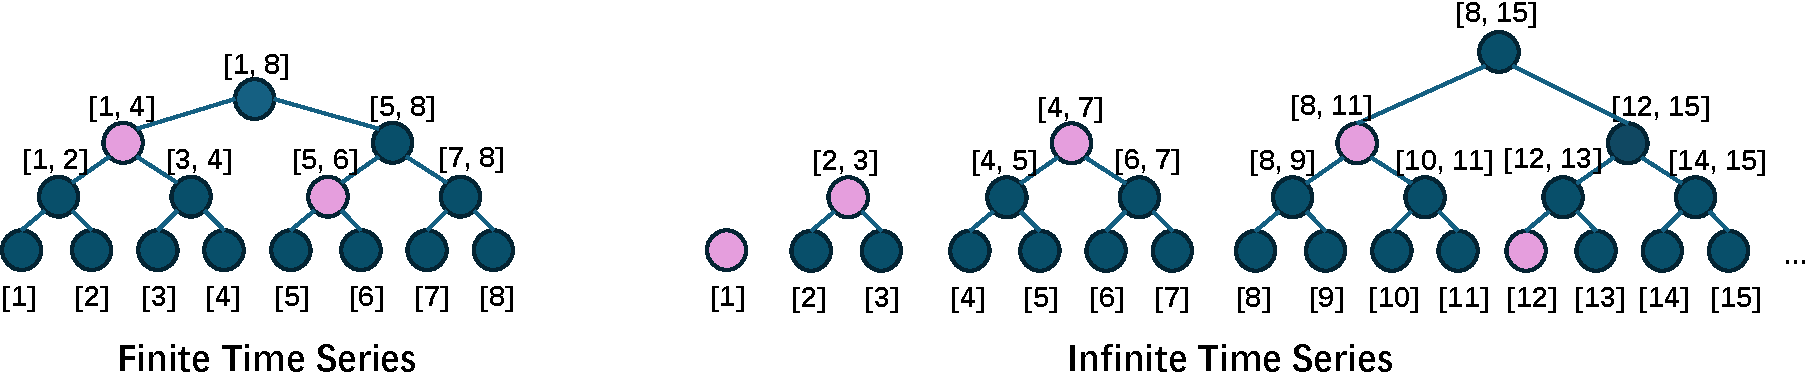
\includegraphics[width=0.8\textwidth]{submissions/submission4/figs/03-count/tree_mechanism-crop.pdf}
%	\caption{For finite time series $[1, 8]$ (i.e., $T=8$), the count query result for the range $[1, 6]$ is specified as $\mathrm{\hat{F}}_{\mathrm{cnt}}(1, [1, 6])=\mathrm{F}_{\mathrm{cnt}}(1, [1, 4])+\mathrm{F}_{\mathrm{cnt}}(1, [5, 6])+2Lap(\frac{\log T+1}
%	{\epsilon})$, where $Lap(b)$ is the Laplace distribution with zero mean. For an infinite time series at timestamp $t$, the mechanism first finds the timestamp $T=2^{\lfloor\log t\rfloor}$ and obtains $\mathrm{\hat{F}}_{\mathrm{cnt}}(1, [1, T])=\mathrm{F}_{\mathrm{cnt}}(1, [1, T])+Lap(\frac{2}{\epsilon})$. Additionally, elements exceeding the power of two (i.e., $[5, 6]$ with length $T'=2$) are processed as a finite time series. Namely, $\mathrm{\hat{F}}_{\mathrm{cnt}}(1, [1, 6])=\mathrm{F}_{\mathrm{cnt}}(1, [1, 4])+Lap(\frac{2}
%	{\epsilon})+\mathrm{F}_{\mathrm{cnt}}(1, [5, 6])+Lap(\frac{\log T'+1}
%	{\epsilon})$.}
 	\caption{Here is an illustration of binary tree mechanism for time series count query under event-level CDP. For finite time series $[1, 8]$ (i.e., $T=8$), the count query result for the range $[1, 6]$ is specified as $\mathrm{\hat{F}}_{\mathrm{cnt}}(v, [1, 6])=\mathrm{F}_{\mathrm{cnt}}(v, [1, 4])+\mathrm{F}_{\mathrm{cnt}}(v, [5, 6])+2Lap(\frac{\log T+1}{\epsilon})$, where $Lap(\cdot)$ is drawn from the Laplace distribution with zero mean. For an infinite time series, multiple binary trees will be constructed. Since a change in any single element only influences one tree, each tree will be allocated an entire privacy budget. The overall privacy budget consumption of the mechanism is $\epsilon$, which can be calculated using parallel composition~\cite{li2017differential}. For example, $\mathrm{\hat{F}}_{\mathrm{cnt}}(v, [1, 12])=\mathrm{\hat{F}}_{\mathrm{cnt}}(v, [1, 1])+\mathrm{\hat{F}}_{\mathrm{cnt}}(v, [2, 3])+\mathrm{\hat{F}}_{\mathrm{cnt}}(v, [4, 7])+\mathrm{\hat{F}}_{\mathrm{cnt}}(v, [8, 11])+\mathrm{\hat{F}}_{\mathrm{cnt}}(v, [12, 12])$.}
	\label{tree_mechanism}
\end{figure}


In addition to the tree-based structure, another approach to handle time series under differential privacy is based on the matrix mechanism~\cite{li2015matrix, henzinger2023almost}.
 Without privacy concerns, a count query $\mathcal{M}$ for binary time series $x$ with length $n$ can be specified as 
\begin{equation}
	\mathcal{M}(x) = Mx= \begin{bmatrix}\nonumber
		1 & 0 & 0 & \cdots  \\
		1 & 1 & 0 & \cdots \\
		1 & 1 & 1 & \cdots \\
		\vdots& \vdots & \vdots & \ddots
	\end{bmatrix} x = \begin{bmatrix}
	x_1\\
	x_1+x_2 \\
	\vdots \\
	\sum_{1}^{n} x_i
\end{bmatrix}.
\end{equation}
Based on this formulation, the matrix mechanism is employed to release data streams under $(\epsilon, \delta)$-DP for further error reduction. Given a workload matrix $M$, the strategy matrix $R$ and reconstruction matrix $L$ are first constructed, denoted as $M=LR$. The strategy matrix $R$ is utilized to pre-process the input $x$. After adding a Gaussian noise vector $z$ to the processed term $Rx$, a post-processing step $L$ is applied. In summary, for an input time series $x\in \mathbb{R}^n$, the matrix mechanism is denoted as 
\begin{equation}\nonumber
	\mathcal{M}_{L, R}(x)=L(Rx+z),
\end{equation}
where $z\sim N(0, \lVert R \rVert^2_{1\to 2}C^2_{\epsilon, \delta}\textbf{I})$ to ensure $(\epsilon, \delta)$-DP, $\lVert R \rVert^2_{1\to 2}$ is the maximum of the 2-norm of the columns of the strategy matrix $R$. The additive mean squared error $\mathrm{err}_{\ell^2_2}$ of the matrix mechanism is 
\begin{equation}\nonumber
	\mathrm{err}_{\ell^2_2}(\mathcal{M}_{L, R}, \mathcal{M}, n) =  \max_{x \in \mathbb{R}^n} \mathbb{E}\left[\frac{1}{n} \left\|  \mathcal{M}_{L, R}(x) - \mathcal{M}(x) \right\|_2^2 \right]=\frac{1}{n} trace(L^TL)\lVert R \rVert^2_{1\to 2}C^2_{\epsilon, \delta}.
\end{equation}
Hence, the matrix mechanism can be regarded as an optimization problem. For more comprehensive information, we recommend reading the work by Henzinger et al.~\cite{henzinger2023almost}.

\subsection{Advanced Queries Based on Count Queries}
 \begin{table}[h]
	\renewcommand\arraystretch{1.5}
	\scriptsize
	\begin{tabular}{cccccc}% 其中,tabular是表格内容的环境;c表示centering,即文本格式居中;c的个数代表列的个数
		\toprule %[2pt]设置线宽     
		\textbf{Query}&\textbf{Ref.} & \textbf{Type}&\textbf{Privacy Level}  & \textbf{Method Primitive}& \textbf{Error Bound} \\ %换行
		\midrule %[2pt]  
		\multirow{4}{*}{\parbox{3.2cm}{Binary  Counting}}&\cite{dwork2010differential} & finite  &event-level CDP & binary tree mechanism & $O(\frac{1}{\epsilon}\cdot (\log^{1.5}t))$\\
		&\cite{chan2011private}&infinite &event-level CDP & binary tree mechanism & $O(\frac{1}{\epsilon}\cdot (\log^{1.5}t))$\\
		&\cite{dong2023continual} & infinite  &user-level CDP & binary tree mechanism & $O(\frac{\kappa(D_t)}{\epsilon}\cdot \log^{1.5}t\cdot \log^{1+\theta}(\kappa(D_t)))$ \\
		&\cite{henzinger2023almost}  & infinite  & event-level ($\epsilon, \delta$)-CDP& matrix mechanism & $O(\frac{4}{\epsilon^2}(\frac{4}{9}+\ln (\frac{1}{\delta}\sqrt{\frac{2}{\pi}}))(1+\frac{\ln(4n/5))}{\pi})^2)$ \\
		\hline
		\multirow{2}{*}{\parbox{3.2cm}{Frequency Estimation}}& ~\cite{cardoso2022differentially} & finite & event-level zCDP & multi-branch tree& $O(\tau\log T\sqrt{2(s+1)(t-1)\log(6T/\beta)})$\\
		&\cite{dong2023continual} & infinite  &user-level CDP & binary tree mechanism & $O(\frac{\kappa(D_t)}{\epsilon\theta}\cdot \log^{1+\theta}(\kappa(D_t)))\cdot \log(tR/\beta)$ \\
		\hline
		\multirow{1}{*}{\parbox{3.2cm}{Distinct Elements Counting}}&\cite{knop2023counting} & finite  &user-level CDP & bipartite maximum matching & $O(\frac{\ell_*}{\epsilon}\log(\frac{\ell_{\max}}{\beta})$\\
		\bottomrule %[2pt]     
	\end{tabular}
	\caption{A brief summary of count-based queries, where $t$ indicates the current timestamp, $T$ is the length of the time series, $D$ represents the dataset, $\kappa(D_t)$ denotes the maximum number of elements contributed by any user, $\tau$ is the privacy level of zero-concentrated differential privacy (zCDP)~\cite{bun2016concentrated}, $\theta$ is any small constant, $\ell$ is the sensitivity ($\ell_*$ represents the bounded sensitivity), and $\beta$ is the confidence parameter. \tablefootnote{The error bound of~\cite{henzinger2023almost} in the table is the $L_2$ norm error.}}
	\label{count_query}
\end{table}
Based on basic binary count queries, numerous other types of count queries have been proposed, including frequency estimation, frequency moment estimation, and distinct element counting. A brief summary of the literature is presented in Table~\ref{count_query}.
Cardoso et al.~\cite{cardoso2022differentially} introduced differentially private histograms in the continual observation model with an unknown domain. To facilitate practical implementation, the authors propose a mechanism that continually returns a noisy histogram by aggregating counts at each round and adding noise to them.
Dong et al. \cite{dong2023continual} proposed a mechanism to estimate frequency under user-level CDP. Since a user may contribute multiple elements to the time series, the mechanism first estimates each user's contribution and then applies a truncation process to retain only a limited number of elements per user, marking subsequent items as invalid. Furthermore, the proposed approach reduces the domain of elements to further enhance the utility of frequency estimates. 
The work by~\cite{knop2023counting} proposes a method to estimate the number of distinct elements in a time series, and obtain the bounds on the true number of unique elements. The paper models the dataset as a bipartite graph and reduces the unique counting process to a max-flow problem, allowing the utilization of standard algorithms for bipartite maximum matching to solve unique counting problem.
Furthermore, Kalemaj et al. \cite{kalemaj2023counting} proposed a mechanism that achieves a logarithmic error bound for releasing distinct elements with insertions and deletions in a finite time series, under item-level differential privacy, which considers neighboring datasets differing by more than one element deletion.
Epasto et al.~\cite{epasto2023differentially} presented the first work to release differentially private $\ell_p$ frequency moments, denoted as $\sum_i f_i^p$. Notably, when $p=1$, the frequency moment reduces to distinct counting.
Practically, Zhang et al.~\cite{zhang2023differentially} propose DP-SQLP, the first differentially private stream aggregation processing system, which has been implemented for Google Shopping and is planned for future application to Google Trends.





\subsection{Downstream Applications Based on Count Queries}
The application of differential privacy in count queries primarily involves releasing histograms and monitoring anomalies. Recent research~\cite{koga2022privacy} has demonstrated that employing subsampling and filtering techniques can reduce the sensitivity of real-time series, thereby enhancing the utility of differentially private mechanisms applied to such data. To improve utility, these mechanisms~\cite{fan2013adaptive, fan2013differentially, li2015differentially, wang2017secweb} typically employ sampling to reduce the number of elements needing protection and filtering to mitigate the impact of added noise. Additionally, some mechanisms leverage pufferfish privacy~\cite{liang2020pufferfish, ding2022publishing}, which introduces less noise while achieving similar privacy guarantees. The details of these mechanisms are as follows.
Fan et al.~\cite{fan2013adaptive} introduced a mechanism for collecting count query results under the FAST framework, which employs filtering and adaptive sampling techniques to satisfy CDP.   In a separate work, Fan et al.~\cite{fan2013differentially} applied the FAST framework for anomaly detection, specifically for detecting epidemic outbreaks.
Li et al.~\cite{li2015differentially} proposed a mechanism that only releases the histogram when it significantly differs from previous values, with the threshold adjusted according to feedback from the control system.
Wang et al.~\cite{wang2017secweb} proposed a framework called SecWeb, following the idea of FAST under $w$-event level differential privacy. In addition to adaptive sampling and filtering, SecWeb incorporates dynamic grouping and injects Laplace noise based on the groups rather than individual elements.
Wang et al.~\cite{wang2018privacy} proposed the first mechanism to achieve almost local differential privacy (LDP) under the $w$-event privacy model. Their approach involves employing multiple agents to collect data from users and release sanitized data to an untrusted third party.
Liang et al.~\cite{liang2020pufferfish} introduced a mechanism for releasing web browsing histograms under the pufferfish privacy framework, which is beneficial for perturbing correlated data. Their proposed mechanism includes a model to quantify privacy leakage arising from temporal correlations and presents three strategies to enhance the model's efficiency: bounding the number of secret pairs, limiting the session length, and avoiding repetitive computations. 
Ding et al.~\cite{ding2022publishing} proposed a mechanism within the framework of pufferfish privacy to make the time and occurrence of an element indistinguishable.



Based on count queries, mechanisms proposed under the local differential privacy (LDP) framework are commonly used to estimate statistics. 
%A line of work under event-level privacy has been proposed based on local differential privacy in the temporal setting (TLDP). Under this framework, the mechanisms perturb the time order instead of directly perturbing the values, resulting in the retention of the original values. Ye et al.~\cite{ye2023stateful} proposed an improved version of their previous work~\cite{ye2021beyond} that employs bi-directional perturbation to reduce collisions. These two mechanisms are used for frequency counting on the 'increase' or 'decrease' of daily stock prices. Mao et al.~\cite{mao2023utility} proposed mechanisms based on the work by Ye et al.~\cite{ye2021beyond} for anomaly detection, where the utility is enhanced by decreasing collisions through the condensed local differential privacy framework introduced by Gursoy et al.~\cite{gursoy2019secure}.
To conserve the privacy budget under LDP, a memoization technique~\cite{erlingsson2014rappor} was proposed, which stores sanitized versions of all values for further release. ~\cite{ding2017collecting} improved upon memoization by incorporating hashing. However, memoization may leak privacy in the presence of a knowledgeable adversary who can potentially derive changes without prior knowledge. Xue et al.~\cite{xue2022ddrm} introduced a difference tree-based mechanism that applies fresh perturbation at each timestamp under user-level privacy, enabling the aggregation of statistics without violating changing points. Additionally, ~\cite{arcolezi2022frequency} proposed a method to reduce the item domain, thereby enhancing utility. 
Beyond memoization based methods, He et al.~\cite{he2022ordinal} proposed a privacy budget allocation strategy to enhance the utility of frequency release under $w$-event level condensed local differential privacy (CLDP)~\cite{gursoy2019secure}. In their approach, the allocated privacy budget depends on the predicted elements, determined via a proportional-integral-derivative (PID) controller.
In other applications, 
Feng et al.~\cite{feng2023dpi} proposed a mechanism to estimate the distribution of infinite time series while satisfying user-level differential privacy. Their approach achieves reasonable utility by bounding privacy leakage and optimizing the allocation of the privacy budget.
Li et al.~\cite{li2024local} introduced the first work on collecting the top-$k$ items from a time series while satisfying event-level local differential privacy and adhering to a bounded memory space constraint. Their proposed mechanisms are based on the HeavyGuardian data structure, which maintains the frequently occurring elements while evicting the infrequent ones.
Additionally, Gu et al.~\cite{gu2023differential} introduced a mechanism under pattern-level privacy, which is similar to $w$-event level privacy but does not require successions. To privately release critical patterns (i.e., subsequences of elements in a time series), their mechanism perturbs the existence of each element, thereby providing a privacy guarantee.






\section{Differential Privacy for Sum/Mean Queries}\label{sec4}
This section provides a comprehensive review of the literature concerning sum and mean queries within the differential privacy framework. It explores the concept of sum/mean queries, the basic queries, and the downstream applications.
\subsection{Essential Information of Sum/Mean Queries}
While preserving the occurrence of an element in a time series is important, maintaining the accuracy of the element's value is equally crucial. To ensure precise results for queries such as sum or mean, small deviations in the perturbation process are necessary. Since the mean is directly correlated to the sum, we discuss sum and mean queries together.

The sum query can be denoted as 
\begin{equation}\nonumber
	\mathrm{F}_{sum}(T, S)=\sum_{i=1}^{T}S_i,
\end{equation}
where $T$ represents the timestamp for sum release and $S$ is the corresponding time Series. The range query on sum is 
\begin{equation}\nonumber
	\mathrm{F}_{rsum}((T_1, T_2), S)=\sum_{i=T_1}^{T_2}S_i,
\end{equation}
where $(T_1, T_2)$ represents the query range, and $S$ is the corresponding time Series.

As for the mean query, it can be denoted as
\begin{equation}\nonumber
	\mathrm{F}_{mean}(T, S)=\frac{1}{T}\sum_{i=1}^{T}S_i,
\end{equation}
where $T$ represents the timestamp for mean release, and $S$ is the corresponding time Series.
Another common mean query is to release the mean at a timestamp from users' time series, 
\begin{equation}\nonumber
	\mathrm{F}_{rtm}(t, S)=\frac{1}{n}\sum_{i=1}^{n}S_t^{u_i},
\end{equation}
where $S_t^{u_i}$ represents the value at timestamp $t$ from the user $u_i$, and $n$ is the number of users.


\subsection{Basic Sum/Mean Queries}
\begin{table}[h]
	\renewcommand\arraystretch{1.5}
	\scriptsize
	\begin{tabular}{cccccc}% 其中,tabular是表格内容的环境;c表示centering,即文本格式居中;c的个数代表列的个数
		\toprule %[2pt]设置线宽     
		\textbf{Query}&\textbf{Ref.} & \textbf{Type}&\textbf{Privacy Level}  & \textbf{Method Primitive}& \textbf{Error Bound} \\ %换行
		\midrule %[2pt]  
		\multirow{1}{*}{\parbox{3.2cm}{Sum}}&\cite{dong2023continual} & infinite  &user-level CDP & binary tree mechanism & $O(\frac{\varphi(D_t)}{\epsilon\theta}\cdot \log^{1.5}(tR)\cdot \log^{1+\theta}(\varphi(D_t))\cdot\log(1/\beta))$\\
		\hline
		\multirow{2}{*}{\parbox{3.2cm}{Window Sum}}&\cite{bolot2013private} & finite  &event-level CDP & binary tree mechanism & $O(\frac{1}{\epsilon}\log W\frac{1}{\beta})$\\
		&\cite{henzinger2024unifying} & finite  &event-level ($\epsilon, \delta$)-CDP & matrix mechanism & $O(2\sigma^2_{\epsilon, \delta}\Delta^2(1+\frac{\log W}{\pi}+\frac{2}{W})^2)$\\
		\hline
		\multirow{2}{*}{\parbox{3.2cm}{Exponential Decay Sum}}&\cite{bolot2013private} & finite  &event-level CDP & binary tree mechanism & $O(\frac{1}{\epsilon}\log \frac{\alpha}{1-\alpha}\frac{1}{\beta})$\\
		&\cite{henzinger2024unifying} & finite  &event-level ($\epsilon, \delta$)-CDP & matrix mechanism & $O(\sigma^2_{\epsilon, \delta}\Delta^2(1+\frac{1}{\pi}S_{T, 2\alpha})^2)$\\
		\hline
		\multirow{2}{*}{\parbox{3.2cm}{Polynomial Decay Sum}}&\cite{bolot2013private} & finite  &event-level CDP & binary tree mechanism & $\Omega(1-\frac{\epsilon^{c-1}}{\log^{c-1}(1/\beta)})$\\
		&\cite{henzinger2024unifying} & finite  &event-level ($\epsilon, \delta$)-CDP & matrix mechanism & $O(\sigma^2_{\epsilon, \delta}\Delta^2(1+\frac{H_{T, 2c}-1}{4})^2)$\\
		\bottomrule %[2pt]     
	\end{tabular}
	
	\caption{The table provides a brief summary of sum-based queries,  where $\varphi(D_t)$ denotes the maximum contribution from any user at time $t$, $\theta$ is a small constant,  $W$ is the window length, $\beta$ is the confidence parameter, $\alpha$ indicates the exponential decay parameter, $c$ represents the polynomial decay parameter, $H_{T, 2c}$ is the generalized Harmonic sum, $S_{T, 2\alpha}$ is a defined series sum with $\alpha>1$.\tablefootnote{The error bound of~\cite{henzinger2024unifying} in the table is the $L_2$ norm error.}} 
	\label{sum_query}
\end{table}


There have proposed a line of work to release sum/mean queries under differential privacy, with a brief summary provided in Table~\ref{sum_query}.
The pioneering work by Bolot et al.~\cite{bolot2013private} was the first to study the continual decaying sums problem. They explored three variants: the window sum (range sum query), which releases the sum of $W$ consecutive elements; the exponential decay sum, which releases the sum of elements weighted by an exponential function; and the polynomial sum, which releases the sum of elements weighted by a polynomial function. 
Henzinger et al.~\cite{henzinger2024unifying} also investigated the continual decaying sum problem. Their work introduced the use of the Gaussian mechanism for adding noise and derived tighter error bounds. 
In contrast, Dong et al.~\cite{dong2023continual} addressed sum queries by reducing them to count queries, as their approach could only handle the latter. For each timestamp with value $x_i$, they expand it into $R$ steps, where the first $x_i (w.l.o.g., x_i<R)$ steps are filled with $1$, and the remaining steps are filled with a special symbol $\perp$. However, this method requires prior knowledge of the maximum value $R$ that can occur in the time series.
~\cite{wang2021continuous} proposed a method for answering sum queries with a threshold under a multi-branch tree structure. The threshold is optimized based on the expected squared error between the true result and the estimated one.   Their proposed mechanism cannot handle infinite time series, so they claim that most queries focus on a limited range, allowing for truncation of the infinite time series. Additionally, their work introduced the first mechanism to release time series under LDP with a threshold for value truncation. 
Instead of directly perturbing the values, the mechanisms proposed by Ye et al.~\cite{ye2021beyond, ye2023stateful} perturb the temporal order. This approach makes them naturally adaptable for sum/mean queries while preserving the original values. These methods demonstrate superior performance for calculating moving averages.

%\subsection{Privacy Budget Allocation Strategies for Sum/Mean Queries}
%In contrast to count queries, sum/mean queries are more sensitive to the actual values, making them more critical from a privacy perspective. Consequently, various privacy budget allocation strategies have been proposed following the introduction of $w$-event level privacy~\cite{Kellaris14}. Although the work~\cite{Kellaris14} is for time series release, the introduced strategies are inspirational for sum/mean queries. The budget distribution strategy, which allocates the privacy budget in an exponentially decreasing manner, and the budget absorption strategy, which allocates the budget uniformly and absorbs invalid allocations. While the budget absorption strategy salvages the privacy budget for invalid allocations, it can lead to compulsory empty outputs when the sum of the privacy budget exceeds the predefined value. 
%Building upon the ideas of the budget distribution and absorption strategies, Ren et al.~\cite{ren2022ldp} proposed corresponding strategies under the local differential privacy (LDP) framework. To mitigate the utility degradation caused by dividing the privacy budget, the authors instead divide the users, with each user reporting only one timestamp within a $w$-length window. 
%To enable real-time computation of the mean at any timestamp from users' time series under $w$-event LDP, Wang et al.~\cite{wang2020towards} proposed sampling strategy to select important elements and privacy budget allocation strategy according to the importance of the elements. However, the sampling process may inadvertently reveal some private information due to the intentional selection.

\subsection{Downstream Applications Based on Sum/Mean Queries}
Due to utility considerations, existing mechanisms for downstream applications based on sum and mean queries primarily operate under event-level privacy or $w$-event level privacy.
Perrier et al.~\cite{perrier2018private} introduced a differentially private mechanism for publishing statistics of real-valued time series under event-level privacy, such as moving averages derived from energy data collected through smart meters. Their approach addresses scenarios where the bound on observations is either overly conservative or unknown, which is crucial for real-time monitoring applications. The proposed mechanism optimizes utility by scaling the added noise to the threshold value instead of a potentially larger bound, thereby improving accuracy.
To enable real-time computation of the mean at any timestamp from users' time series under $w$-event LDP, Wang et al.~\cite{wang2020towards} proposed sampling strategy to select important elements and a privacy budget allocation strategy according to the importance of the elements. However, the sampling process may inadvertently reveal some private information due to the intentional selection.
Kurt et al.~\cite{kurt2022online} proposed an online anomaly detection method for networks based on the cumulative sum algorithm, satisfying event-level $(\epsilon, \delta)$-differential privacy. Their approach adds noise to the statistic at each timestamp from each network node, operating under event-level privacy, and then derives the mean from the data of all nodes. This allows for detecting anomalies by monitoring changes in the released means.











\section{Differential Privacy for Time Series Release}\label{sec5}
Time series release aims to publicly share private time series while preserving privacy. Value perturbation methods add noise to the data values, often using sampling and adaptive budget allocation for utility. While temporal perturbation methods dispatch elements across timestamps to obfuscate event timings, avoiding value distortion but risking empty releases or collisions.

\subsection{Value Perturbation Based Methods}
Time series release aims to directly publicize the time series for downstream tasks. Since time series release focuses on preserving the accuracy of values, privacy budget allocation is critical for controlling added noise and minimizing distortion. Therefore, a sampling-based method is often employed to select crucial elements according to the tasks, reducing the number of points requiring privacy budget allocation and enhancing utility. Additionally, to further improve the utility of the released data, a post-processing step can be adopted to correct the noisy data using prior knowledge. The outline of time series release is summarized in Fig.~\ref{release_process}.
\begin{figure}[h]
	\centering
	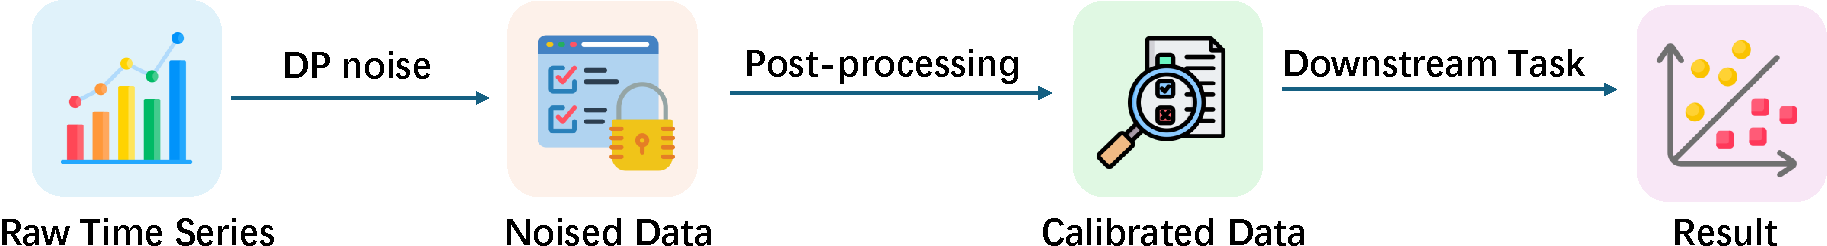
\includegraphics[width=0.8\textwidth]{submissions/submission4/figs/05-release/data_release-crop.pdf}
	\caption{The outline of time series release under differential privacy.}
	\label{release_process}
\end{figure}

\subsubsection{Privacy Budget Allocation Strategies}
User-level privacy protects the elements from any user but requires a larger privacy budget for reasonable utility, particularly challenging for time series release. Conversely, event-level privacy safeguards individual elements, yet may not suffice for comprehensive privacy guarantees. To balance the privacy levels,  
Kellaris et al.~\cite{Kellaris14} first proposed $w$-event level privacy under CDP. By leveraging $w$-event level privacy, sanitized time series can offer better privacy guarantees than event-level privacy and higher utility than user-level privacy. To optimize the advantages of $w$-event level privacy, Kellaris et al. \cite{Kellaris14} proposed two privacy budget allocation strategies. Building upon the ideas of the budget distribution and absorption strategies in \cite{Kellaris14}, Ren et al.~\cite{ren2022ldp} proposed corresponding strategies under LDP framework. To mitigate the utility degradation caused by dividing the privacy budget, the authors divide the users instead, with each user reporting only one timestamp within a $w$-length window. 
Several sampling-based methods have been developed to reduce the number of elements requiring a privacy budget, with adaptive budget allocation based on element importance. 
Wang et al.~\cite{wang2016rescuedp} introduced RescueDP, a scheme for real-time publishing of spatio-temporal crowd-sourced data with $w$-event level CDP, integrating adaptive sampling, privacy budget allocation, dynamic grouping, perturbation, and filtering techniques. The adaptive sampling component adjusts sampling rates based on data changes, ensuring efficient resource utilization. The privacy budget allocation mechanism dynamically distributes the privacy budget for sampling points across successive timestamps. Zhang et al.~\cite{zhang2017re} proposed Re-DPoctor, a real-time health data releasing scheme ensuring $w$-event level CDP, enhancing utility with a partition algorithm safeguarding health data patterns and improving privacy through adaptive sampling and budget allocation.
He et al.~\cite{he2022ordinal} introduced a new privacy concept using condensed local differential privacy (CLDP)~\cite{gursoy2019secure} for $w$-event level privacy, aiming to enhance utility. They save privacy budget from empty releases and reallocate it to released elements, and utilize a PID controller-based method for adaptive budget allocation. However, this approach may inadvertently disclose private information through omitted empty points.

\subsubsection{Optimization Strategies}
Leveraging the correlations present in time series, the pre-processing or post-processing methods can be applied to improve the utility of the perturbed data.
Ren et al.~\cite{ren2018textsf} addressed privacy challenges in high-dimensional crowdsourced data by proposing LoPub, an LDP data publication algorithm under event-level privacy. They use expectation maximization (EM) and Lasso regression to efficiently estimate multivariate joint distributions, identifying attribute correlations to reduce data dimensionality for distribution learning speed and utility improvements.
Wang et al.~\cite{wang2019locally} proposed the methods, LoCop and DR\_LoCop, for releasing high-dimensional crowdsourced data under event-level LDP. The methods comprise four integrated components: a transformation component that ensures LDP by hashing and randomizing the data, an estimation component that infers probability distributions from the resulting Bloom filter strings, a computation component that derives marginal distributions and captures dependencies among dimensions, and a sampling component that generates a new synthetic dataset based on the computed distributions and dependencies. 
Fioretto and Hentenryck~\cite{fioretto2019optstream} introduced OptStream,  a method for releasing time series under $w$-event level, which extends to handling hierarchical streams like energy profiles, making it applicable beyond its original energy domain. OptStream involves four key steps: sampling points for private measurement, perturbing them for privacy, reconstructing non-sampled points, and post-processing with convex optimization to improve accuracy by redistributing added noise.
Zhang et al.~\cite{zhang2022differentially} introduced a method for releasing differentially private sequential data using first-order autoregressive processes under user-level privacy. Their approach estimates unreleased data from previously released data by leveraging learned correlations, without requiring prior knowledge. The estimated data is combined with the observed data and perturbed with calibrated noise at each timestamp, facilitating real-time data release.
Li et al.~\cite{li2023locally} proposed a framework for locally private stream data release that employs shuffling and subsampling techniques. Their approach maintains utility in the context of continual data collection by sampling a subset of users at each timestamp. An optimal sample size is determined to reduce redundant data and enhance utility, and the framework incorporates pre-processing within the shuffler to mitigate bias arising from distributed sampling. 
Besides pre- or post-processing methods, Bao et al.~\cite{bao2021cgm} proposed a mechanism based on the assumption of data fluctuation. Since time series may not change significantly over time, this mechanism formalizes the correlation between elements, allowing a later element to be represented by previous elements. To protect privacy, noise is added to the correlation.

\subsection{Synthesis Based Methods}
Directly releasing users' data poses significant risks of privacy breaches. An alternative approach is to train a synthesis model under strict privacy conditions and then release the data generated by this model for downstream tasks. To synthesize time series data under DP, one method involves first estimating the relevant statistics and then generating the synthetic data based on these estimations. Additionally, the advent of Generative Adversarial Networks (GANs) under DP~\cite{xie2018differentially, jordon2018pate} has facilitated the use of deep learning algorithms to generate data, thereby enhancing both privacy protection and data accuracy.

\subsubsection{Synthesis Based on Statistics}
Synthesis mechanisms based on statistical features first capture the statistical characteristics from datasets under DP. Subsequently, new data is generated according to these estimated statistics. He et al.~\cite{he2024online} introduced an efficient polynomial-time algorithm for generating online differentially private synthetic data under event-level privacy from a continuous time series within the hypercube $[0, 1]^d$. The algorithm achieves near-optimal accuracy bounds in $1$-Wasserstein distance and extends previous work to include Lipschitz queries. By utilizing an online hierarchical partitioning approach and a novel Inhomogeneous Sparse Counting Algorithm, the method maintains strong privacy guarantees while ensuring high utility for infinite time horizons. To achieve a higher privacy level, 
Bun et al.~\cite{bun2024continual} focused on generating differentially private synthetic data through statistical estimation under user-level CDP. They proposed algorithms that maintain the accuracy of fixed time window and cumulative time queries, ensuring minimal error while preserving privacy. Their approach involves a two-stage process that combines noisy estimates with post-processing techniques to ensure consistency and accuracy in synthetic data generation.



% GAN
\subsubsection{Synthesis Based on Generative Models}
In addition to statistics-based mechanisms, another method for synthesizing time series is through Generative Adversarial Networks (GANs). Unlike other data types, time series requires consideration of temporal correlations. 
Frigerio et al.~\cite{frigerio2019differentially} presented a framework for releasing high-quality open data while ensuring user privacy through DP, addressing both continuous and discrete data. By leveraging deep learning and generative models with long short-term memory networks, the framework maintains data utility and correlations, introducing innovations such as clipping decay to optimize performance.
Wang et al.~\cite{wang2020part} introduced PART-GAN, a privacy-preserving generative model designed for time series augmentation and sharing. PART-GAN combines Conditional and Temporal Generative Adversarial Networks (CT-GAN) with differential privacy mechanisms, enabling the generation of unlimited synthetic data that addresses issues of incomplete and irregularly sampled time series.
Torfi et al.~\cite{torfi2022differentially} proposed a mechanism to generate high-quality synthetic health record data while ensuring privacy using R\'enyi Differential Privacy (RDP). Their framework combines convolutional autoencoders and convolutional generative adversarial networks (CGAN) to effectively handle both discrete and continuous data, preserving temporal and feature correlations.
For specific applications, Lamp et al.~\cite{lamp2024glucosynth} introduced GlucoSynth, a novel privacy-preserving GAN framework designed to generate high-quality synthetic glucose traces while maintaining strong differential privacy guarantees. By focusing on preserving the relationships among glucose events (motifs) and temporal dynamics, GlucoSynth addresses the unique challenges of synthesizing glucose data.





\subsection{Discussion}
The aforementioned release mechanisms modify the values of the original time series, which can degrade utility in value-critical scenarios. For elements in a time series where occurrence indicates more sensitive information, temporal perturbation can be employed to avoid distorting the original values. Ye et al.~\cite{ye2021beyond} first proposed a method to achieve temporal perturbation in the local setting, maintaining the privacy guarantee while enhancing utility.
\begin{figure}[htbp]
	\centering
	\begin{minipage}{0.4\textwidth}
		\centering
		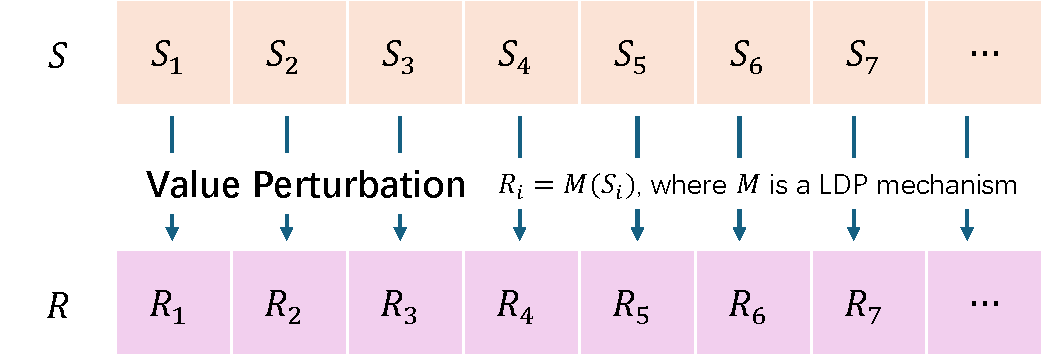
\includegraphics[width=\linewidth]{submissions/submission4/figs/05-release/value_perturbation-crop.pdf}
	\end{minipage}\hspace{0.55in}
	\begin{minipage}{0.4\textwidth}
		\centering
		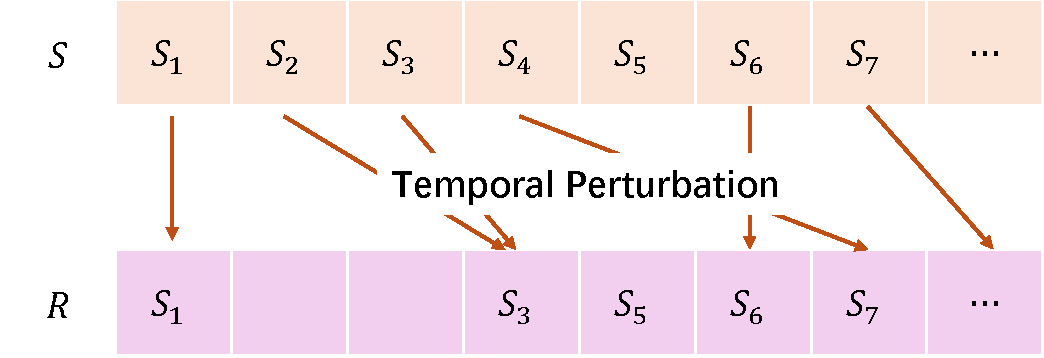
\includegraphics[width=\linewidth]{submissions/submission4/figs/05-release/temporal_perturbation-crop.pdf}
	\end{minipage}
	\caption{Value perturbation-based methods will perturb the original values by adding DP noise. In contrast, temporal perturbation-based methods will dispatch the values to corresponding timestamps for release.}
	\label{vptp}
\end{figure}
As illustrated in Fig.~\ref{vptp}, unlike value perturbation that directly modifies the original values by adding LDP noise, temporal perturbation dispatches elements across different timestamps. This obfuscates the precise occurrence times, preventing adversaries from determining the exact event timings. However, temporal perturbation can lead to issues such as delayed releases, empty releases (where no elements are dispatched to certain timestamps), and element substitutions, resulting in missing data.  To address these issues,  Ye et al.~\cite{ye2023stateful} proposed a bi-directional perturbation mechanism that eliminates collisions during the dispatching process, ensuring that elements are only delayed. Furthermore, Mao et al.~\cite{mao2023utility} extended the definition to a metric-based version tailored for anomaly detection, aiming to reduce collisions involving anomalous elements.  However, these proposed mechanisms~\cite{ye2021beyond, ye2023stateful, mao2023utility} primarily address event-level privacy concerns, leaving room for enhancements to achieve higher levels of privacy.





















\section{Differential Privacy for Location Based Services}\label{sec6}
% definition of trajectory
Location Based Service (LBS) is a crucial application of mobile computing that provides personalized services based on users' geographical locations. These services, ranging from navigation assistance to location-based recommendations, require continuous collection and analysis of users' location data, often in the form of trajectories.

A trajectory is a specific type of time series that comprises spatial-temporal data. 
It can be regarded as a sequence of time-ordered points, denoted as $T=\{p_1, p_2, \cdots, p_{T}\},$ where $p_i$ represents a location and $T$ is the length of the trajectory. 
Compared with other time series, the correlations within trajectory data are more pronounced due to the constraints imposed by spatial variation. Regarding privacy levels for trajectory data, location privacy corresponds to event-level privacy, providing protection for individual locations, whereas trajectory privacy safeguards the entire trajectory.

In this section, we introduce mechanisms for handling trajectory data under differential privacy, organized according to utility improvement in location perturbation, privacy preservation against temporal correlation, and trajectory release. These mechanisms ensure that the privacy of individual locations and movements is preserved while maintaining the utility of the data for analysis and service provision.

% geo-indistinguishablility 
\subsection{Location Perturbation Based on Geo-indistinguishability}
%Geo-indistinguishability~\cite{andres2013geo} is designed to enhance utility in location perturbation. 
For meaningful outputs in LBS, the perturbed location should not deviate excessively from the actual one.   As illustrated in Fig.~\ref{geo}, constraining the perturbation domain is essential for improving utility; otherwise, a large perturbation domain yields less useful results. For example, perturbing Paris to London is impractical~\cite{andres2013geo}. Therefore, a metric-based privacy notion, $\epsilon$-geo-indistinguishability, is proposed.  Specifically, a user's level of privacy is defined as $\ell=\epsilon r$, where $r$ is the radius of the perturbation domain, corresponding to $r_i$ in Fig.~\ref{geo}. Here is the formal definition of geo-indistinguishability.
\begin{definition}[Geo-indistinguishability~\cite{andres2013geo}]
	Given any two locations $x$ and $x'$ ($d(x, x')\le r$), a randomized mechanism $M$ satisfies  $\epsilon$-geo-indistinguishability iff
	\begin{equation}\nonumber
		\mathrm{Pr}[M(x)\in Z]\le e^{\epsilon d(x, x')}\mathrm{Pr}[M(x')\in Z],
	\end{equation}
	where $Z\subseteq \mathcal{Z}$ is the possible output domain, where $d(x, x')$ represents a distance measure between $x$ and $x'$.
\end{definition}

\begin{figure}[h]
	\centering
	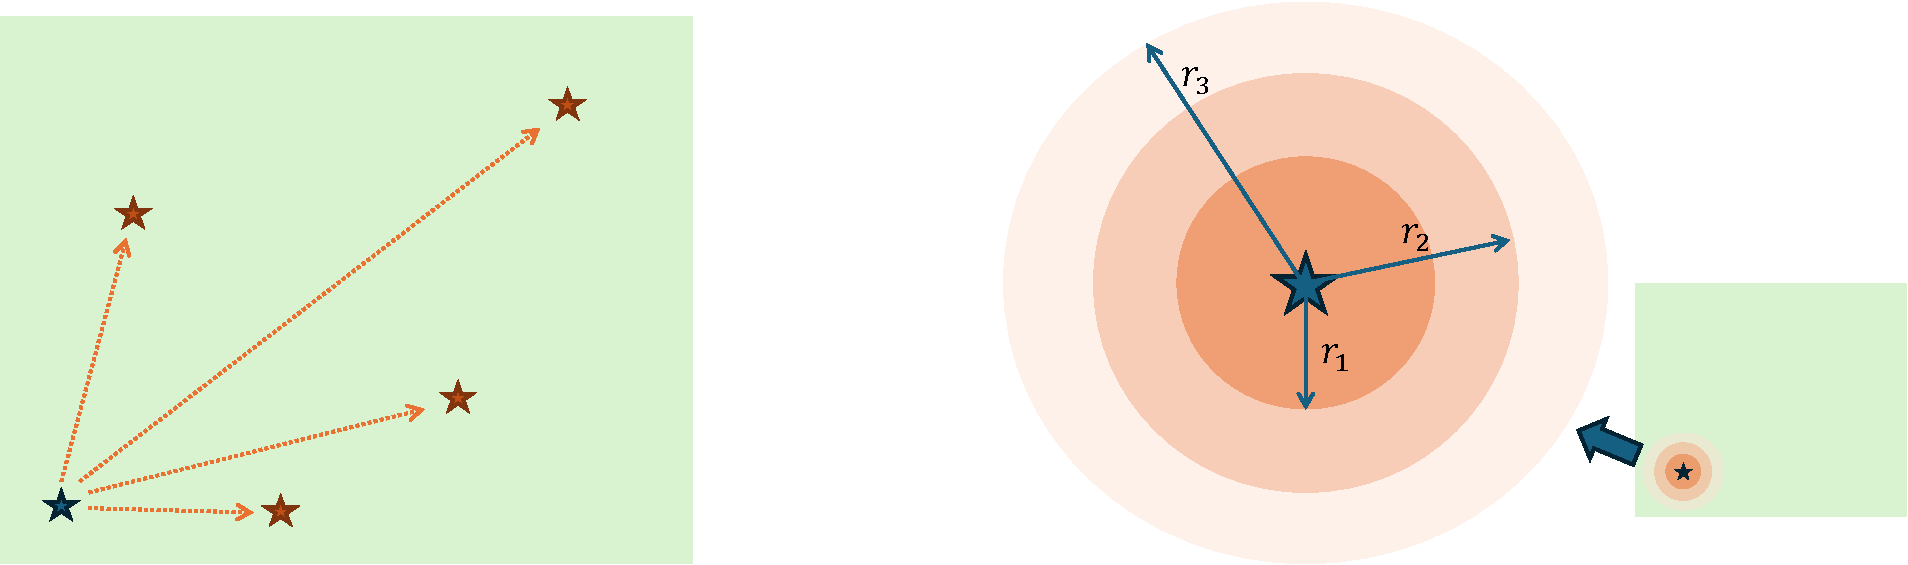
\includegraphics[width=0.8\textwidth]{submissions/submission4/figs/05-release/geo-crop.pdf}
	\caption{A traditional DP mechanism (illustrated in the left-hand figure) involves a perturbation domain (green area) for a location that is typically large, resulting in low utility for the perturbed location. To improve utility while providing useful services, a metric-based privacy notion, geo-indistinguishability, is introduced to control the perturbation (illustrated in the right-hand figure). A smaller distance $r_i$ leads to higher utility but offers less privacy. Therefore, it is important to balance the trade off between utility and privacy when designing mechanisms under geo-indistinguishability.}
	\label{geo}
\end{figure}

Since the inception of geo-indistinguishability, numerous enhancements have been made to improve the privacy notion from various perspectives.
To enhance the calculation efficiency, Bordenabe et al.~\cite{bordenabe2014optimal} proposed a method to optimize the trade-off between geo-indistinguishability and service quality in location privacy, employing linear programming to minimize service quality loss while ensuring optimal privacy guarantees. By reducing the number of constraints from cubic to quadratic, their approach significantly improves computational efficiency.
Building on the concept of geo-indistinguishability, Weggenmann and Kerschbaum~\cite{weggenmann2021differential} introduced the notion of directional privacy, a relaxation of pure differential privacy that performs effectively in the local model. 
To enhance practical utility, Zhao et al.~\cite{zhao2022geo} proposed geo-ellipse-indistinguishability to protect individual location data in directional distribution analysis. This method incorporates the covariance matrix to account for dispersion and orientation of community locations, using elliptical noise instead of circular noise. The proposed mechanisms, based on gamma and multivariate normal distributions, ensure higher probabilities of randomized locations aligning with community location trends while maintaining statistical quality.
Liang and Yi~\cite{liang2023concentrated} further advanced the concept of geo-indistinguishability by introducing concentrated geo-privacy, an update from the CDP version. This approach supports advanced composition mechanisms for high-dimensional data and achieves a lower noise scale, thereby enhancing overall privacy protection while maintaining utility. Zhao and Chen~\cite{zhao2023vector} proposed vector-indistinguishability (vector-ind) to enhance location privacy by preserving distance and direction dependencies between successive locations. They introduced four mechanisms using Laplace and Uniform distributions to achieve vector-ind, maintaining data utility while ensuring CDP.

Several mechanisms have been proposed to address various privacy issues across numerous scenarios based on geo-indistinguishability.  
Yu et al.~\cite{yu2017dynamic} proposed PIVE, a dynamic differential location privacy framework that integrates geo-indistinguishability and expected inference error to protect against inference attacks. PIVE operates in two phases: First, it identifies a protection location set based on user-defined error thresholds and prior knowledge; And then, it generates pseudo-locations within this set, ensuring differential privacy. This approach enables adaptive, personalized privacy settings tailored to individual user needs and location-based service requirements, thereby enhancing both privacy preservation and utility.
Cao et al.~\cite{cao2019priste} extended differential privacy to define $\epsilon$-spatiotemporal event privacy and proposed a framework to quantify its protection level in existing location privacy-preserving mechanisms. They demonstrated their framework by adapting the Planar Laplace Mechanism for geo-indistinguishability to ensure spatiotemporal event privacy while maintaining linear computational complexity.
Niu et al.~\cite{niu2020eclipse} introduced Eclipse, a mechanism that combines geo-indistinguishability, k-anonymity, and expected inference error to protect location privacy against long-term observation attacks. Eclipse obfuscates user locations within an anonymity set, minimizing privacy leakage while maintaining service usability and correctness.
Qiu et al.~\cite{qiu2020location}  tackled the Vehicle-based spatial crowdsourcing Location Privacy (VLP) problem, aiming to minimize travel cost distortion while preserving location privacy over road networks. They redefined geo-indistinguishability based on path distance and approximated the VLP problem as a linear programming formulation through discretization. To improve time efficiency, they proposed a two-layer optimization algorithm and analyzed the trade-off between privacy and quality of service.
Haydari et al.~\cite{haydari2022differentially} proposed a differential privacy-based map-matching algorithm (DPMM) for protecting user privacy in mobility data. DPMM generates privatized link-level location trajectories by incorporating road characteristics such as capacity and functional role. The algorithm adaptively selects the noise level based on link density, effectively balancing privacy preservation and trajectory accuracy.



% temporal correlation
\subsection{Privacy Preservation Against Temporal Correlation}
Due to the intrinsic features of location data, temporal correlations pose significant privacy issues when handling locations. Specifically, an adversary can infer information about a location based on its preceding or succeeding elements. For instance, Shao et al.~\cite{shao2020structured} proposed iTracker, a framework designed to recover multiple trajectories from differentially private data using a structured sparsity model. iTracker leverages interdependencies among locations to enhance recovery accuracy, effectively challenging existing Laplace perturbation-based location protection mechanisms.
To address privacy risks posed by temporal correlations in location data, numerous mechanisms have been proposed.
Xiao and Xiong~\cite{xiao2015protecting} introduced a solution that preserves location privacy with rigorous differential privacy guarantees by proposing $\delta$-location set, which accounts for temporal correlations in location data. They also introduced the sensitivity hull to capture geometric sensitivity in multidimensional space and presented the planar isotropic mechanism (PIM), an efficient location perturbation method that achieves optimal utility while meeting differential privacy requirements.
Cao et al.~\cite{cao2017quantifying} first investigated the privacy loss of CDP mechanisms under temporal correlations and introduced the concept of Temporal Privacy Leakage (TPL). They proposed an efficient algorithm to calculate TPL and designed methods to convert traditional DP mechanisms to ones that mitigate TPL, ensuring privacy over continuous data releases by bounding the leakage within a defined parameter $\alpha$.
Xiao et al.~\cite{xiao2017loclok} proposed LocLok, a system that protects user locations with differential privacy  by modeling temporal correlations using a hidden Markov model and applying PIM for optimal noise addition. LocLok generates possible locations via the Markov model, perturbs them with PIM, and infers true locations within a set of all possible locations, ensuring robust local privacy even when adversaries have access to historical location data.
Liu et al.~\cite{liu2019protecting} protected location privacy by analyzing the impact of temporal-spatial correlations and proposing new privacy definitions, introducing Bayesian-based geo-indistinguishability to better evaluate and enhance privacy levels. Their method optimally allocates noise among spatially and temporally correlated locations, effectively protecting sensitive locations within a trajectory while achieving differential privacy.
Ma et al.~\cite{ma2019real} proposed RPTR under $w$-event level CDP to protect real-time vehicle trajectory data. They employed dynamic sampling and ensemble Kalman filters, utilizing a position transfer probability matrix to infer correlations and ensure accurate predictions while balancing data availability and privacy. Additionally, they introduced a regional privacy weight mechanism to enhance protection in high-density areas, thereby ensuring higher prediction accuracy and adaptability across different scenarios.
Cao et al.~\cite{cao2023differentially} propose a post-processing framework to enhance the utility of differentially private streaming data releases by leveraging temporal correlations. They modeled the problem as a maximum a posterior estimation, transformed it into a nonlinear constrained programming problem, and used a transition matrix to incorporate both probabilistic and deterministic constraints.
Ahuja et al.~\cite{ahuja2023neural} proposed a method to release histogram information from trajectories under user-level CDP. To enhance utility, they introduced a method based on variational autoencoders to refine the histograms by utilizing the correlations of histograms.

\subsection{Trajectory Release Based on Perturbation or Synthesis}
 
% perturbation based release
As location-based services (LBS) become increasingly integral to everyday applications, ensuring the privacy of users while maintaining the utility of location data remains a critical challenge. Various mechanisms have been proposed to address this issue, each focusing on different aspects of location privacy and data utility. 
%A popular direction is to release trajectory data for downstream tasks. Releasing trajectory data while preserving privacy is particularly challenging due to the sensitive nature of location information.
Wang et al.~\cite{wang2022srr} introduced L-SRR, the first LDP framework for location-based services, enhancing utility while ensuring strict privacy. The proposed staircase randomized response mechanism perturbs user locations using optimized probabilities, significantly improving utility for applications such as traffic density estimation and k-nearest neighbor queries.
Cunningham~\cite{cunningham2021real} introduced a locally differentially private mechanism for trajectory data sharing that integrates public knowledge to enhance utility while ensuring privacy. This mechanism perturbs hierarchically-structured n-grams of trajectory data to capture spatio-temporal relationships, leveraging public data without compromising privacy. 
Zhang et al.~\cite{zhang2023trajectory} proposed a trajectory perturbation mechanism under user-level LDP that enhances privacy by using adjacent direction information to connect neighboring points. They introduce a two-stage pivot sampling process utilizing bi-directional clues from pivots, and an anchor-based method to restrict the spatial region of trajectories.

Synthetic trajectory generation has emerged as another promising solution, allowing for the publication of useful data without compromising individual privacy. 
Gursoy et al.~\cite{gursoy2018differentially} presented DP-Star, a framework for publishing trajectory data that ensures differential privacy while maintaining high utility. DP-Star normalizes raw trajectories using representative points, constructs a density-aware grid to preserve spatial densities, and employs a private Markov mobility model to maintain correlations and intra-trajectory mobility. This results in synthetic trajectory datasets that are both privacy-preserving and useful for various data mining tasks.
Moreover, Gursoy et al.~\cite{gursoy2018utility} presented AdaTrace, a scalable location trace synthesizer that achieves statistical privacy, deterministic attack resilience, and strong utility preservation. AdaTrace generates differentially private synthetic traces through a four-phase process: feature extraction, noise injection, and utility-aware synthesis. The synthetic traces preserve utility-critical information and are robust against Bayesian inference, partial sniffing, and outlier leakage attacks, ensuring privacy without significant utility loss.
Du et al.~\cite{du2023ldptrace} introduced LDPTrace, a locally differentially private framework for synthesizing realistic trajectories with minimal computational cost and strong privacy guarantees. LDPTrace captures key movement patterns from users' trajectories, ensuring robust statistical privacy and resilience against attacks. Extensive evaluations demonstrate that LDPTrace generates authentic trajectories without external knowledge, outperforming existing methods in terms of utility and privacy protection.
Hu et al.~\cite{hu2024real} introduced RetraSyn under $w$-event level LDP, aimed at real-time trajectory synthesis while ensuring data privacy. RetraSyn leverages mobility patterns from trajectory streams and incorporates a global mobility model, dynamic update mechanisms, and Markov-based synthesis to generate realistic trajectories. This framework effectively captures complex spatial-temporal contexts and employs adaptive privacy budget allocation strategies, ensuring authenticity and practicality in diverse real-world scenarios.
Sun et al.~\cite{sun2023synthesizing} proposed SPRT, a method for synthesizing private and realistic vehicle trajectories by incorporating geographic structures into differential privacy mechanisms. SPRT constructs a geography-aware grid to capture accurate mobility patterns and defines a moveable constraint based on real-world conditions, enhancing both summary-level statistics and individual-level mobility patterns.





\section{Open Challenges}\label{sec7}
Although many mechanisms have been proposed to handle time series under differential privacy, several issues still need to be addressed. In this section, the challenges will be introduced according to privacy model, potential attacks, data type, and learning based problems.

\subsection{Privacy Model}  
The privacy model is a crucial factor in differential privacy. As aforementioned, there are three privacy levels when handling time series~\cite{Kellaris14}. Event-level privacy guarantees the privacy of a single element in a time series, making it easier to implement since the sensitivity of an individual element in neighboring datasets is simpler to measure. In contrast, user-level privacy provides a higher privacy guarantee and is more practical in real-world applications. However, bounding the sensitivity of a single user's participation is challenging, making the allocation of the privacy budget more complex. Additionally, utility issues become more pronounced when dealing with infinite time series.

Several research works have explored handling infinite time series under user-level privacy with specific conditions. Dong et al.~\cite{dong2023continual} introduced mechanisms for basic queries such as count and sum. These mechanisms are based on event-level privacy approaches and are adapted to user-level privacy by bounding the maximum changes of a single user in a time series. For LDP, Xue et al.~\cite{xue2022ddrm} proposed a mechanism for count queries, but it requires that the time series does not fluctuate significantly. Feng et al.~\cite{feng2023dpi} proposed a strategy that randomly allocates the privacy budget according to a converging sum series.

Therefore, improving the utility of infinite time series under user-level differential privacy is an intriguing future direction. Beyond basic queries, efforts can be made to accommodate specific queries or applications. Key challenges include accurately measuring data sensitivity and effectively allocating the privacy budget. Overcoming these challenges can enhance the practical utility of differential privacy mechanisms for managing infinite time series under user-level privacy.


\subsection{Temporal Correlation Based Attacks}
Compared to other data types, the correlation in time series is more pronounced. Due to the inherent sequential nature of time series, each element is often directly influenced by its predecessors. Various works have employed the Markov model to capture and represent these correlations under DP~\cite{cao2017quantifying, xiao2017loclok, gursoy2018differentially}. In the context of the Markov model, an element is directly influenced only by its immediate neighboring element. Consequently, the influence of previous elements is implicitly carried forward through the chain of direct dependencies between neighboring elements.
Since time series are always modeled explicitly, this simplicity can result in the model overlooking long-term information that extend beyond immediate neighbors. To capture such information, more complex models like the long short-term memory network~\cite{shi2015convolutional} are needed. Moreover, for specific types of time series such as trajectories, public knowledge can introduce additional privacy issues. For example, certain perturbations may be impossible due to physical world limitations. In summary, compared with single data points, elements in time series are at a greater risk of privacy leakage. This suggests a potential direction for research: attacking existing privacy mechanisms by exploiting these correlations and to design new mechanisms that account for the inherent dependencies in time series. 



\subsection{Complex Data Type}
Most current works can only handle simple time series with high utility, such as one value at each timestamp. However, real-world data are more complex, and mechanisms should be designed to handle this complexity. Here are two examples:

First, sensor data are often multi-dimensional and correlated across each dimension. This complexity requires mechanisms capable of managing and analyzing data with multiple interacting variables. Traditional methods that handle single-dimensional elements at each timestamp are insufficient for capturing the nuances of multi-dimensional sensor data. For example, environmental sensors may collect temperature, humidity, and air pressure simultaneously. Analyzing these factors independently can miss critical interactions and patterns, such as how temperature changes might influence humidity levels during users' activities. Therefore, advanced methods must be developed to process and interpret multi-dimensional sensor data effectively.

Second, the element at each timestamp can be intricate. For instance, social networks change over time, making real-time analysis of such dynamic networks complicated. Managing the evolution of relationships and interactions within the network adds a layer of complexity beyond time series analysis. Additionally, privacy concerns in such contexts extend beyond the temporal dimension to include graph privacy, encompassing node-level privacy and edge-level privacy. Mechanisms must account for these additional privacy requirements to ensure data protection while enabling real-time analysis. 

\subsection{Learning Based Problems}
Current DP mechanisms are primarily designed for basic queries, such as count, mean, and frequency. However, time series without privacy concerns are often used for more complex downstream tasks, such as classification and clustering. These tasks require a deeper understanding and manipulation of the data, going beyond simple statistical queries. To accommodate more practical downstream tasks, it is essential to develop DP mechanisms that can support these sophisticated operations effectively, ensuring both the utility and privacy of the data.

A reasonable solution is to generate synthetic time series from the real dataset. Synthetic approach allows the fundamental features of the time series to be captured while protecting the privacy of the underlying data. Since the features of time series are complex and extend beyond basic statistics, traditional statistical methods are insufficient for capturing these intricate patterns. For example, critical patterns such as seasonal trends, cyclic behaviors, and sudden anomalies are vital in time series analysis but are not adequately addressed by basic statistical methods.

Therefore, learning-based methods are preferable for generating synthetic time series. These methods can model and replicate the complex dependencies and structures inherent in time series. For instance, the method proposed by Lamp et al.~\cite{lamp2024glucosynth} for synthesizing glucose traces exemplifies how deep learning can be applied to generate realistic and privacy-preserving synthetic data. Predictably, more and more application-specific mechanisms will be proposed. 


\section{Conclusion}
In this paper, we present a comprehensive survey on handling time series under differential privacy. We begin by introducing the basic concepts of time series and differential privacy, along with relevant definitions. Our survey starts with an exploration of two basic queries: count queries and sum/mean queries. 
For each query type, we first explain the concept of the basic query, then review the core techniques or developments related to the queries, and finally discuss the advanced queries derived from the basic ones. At the end of each query section, we review the downstream tasks based on these queries. 
Subsequently, we introduce mechanisms for time series release,  categorizing them into value perturbation based methods and synthetic generation based methods.
Additionally, we dedicate a separate section to location-based services (LBS), as they are common application scenarios for time series. We review relevant papers for LBS according to two popular privacy issues and the demands of trajectory release. Finally, we illustrate four open challenges and suggest future directions.






\section*{Acknowledgment}
This work was supported by the National Natural Science Foundation of China (Grant No: 62372122, 62072390, and 92270123), the Research Grants Council, Hong Kong SAR (Grant No: 15203120, 15208923 and 15210023),  Shenzhen Key Laboratory of Safety and Security for Next Generation of Industrial Internet\\  (Grant No. ZDSYS20210623092007023) and Guangdong Provincial Key Laboratory of Brain-inspired Intelligent Computation (Grant No. 2020B121201001)



%\bibliographystyle{IEEEtran}
%\bibliography{survey_ref}
\bibliographystyle{unsrt}

\begin{thebibliography}{10}
\itemsep=1pt
\begin{small}
%%%%%%%%%%%%%%%%%%%%%%%%%%%%%%%%%%%%%%%%%%%%%%%%%%%%%%%%%%introduction
\bibitem{hyndman2018forecasting}Hyndman, R. \& Athanasopoulos, G. Forecasting: principles and practice. (OTexts,2018)

\bibitem{gardner2006exponential}Gardner Jr, E. Exponential smoothing: The state of the art—Part II. {\em International Journal Of Forecasting}. \textbf{22}, 637-666 (2006)

\bibitem{shi2015convolutional}Shi, X., Chen, Z., Wang, H., Yeung, D., Wong, W. \& Woo, W. Convolutional LSTM network: A machine learning approach for precipitation nowcasting. {\em Advances In Neural Information Processing Systems}. \textbf{28} (2015)

\bibitem{Dwork2006}
C.~Dwork, ``Differential privacy,'' in \emph{International colloquium on
	automata, languages, and programming}.\hskip 1em plus 0.5em minus 0.4em\relax
Springer, 2006, pp. 1--12.

\bibitem{ye2020local}Ye, Q. \& Hu, H. Local differential privacy: Tools, challenges, and opportunities. {\em International Conference On Web Information Systems Engineering}. pp. 13-23 (2020)

\bibitem{Yang2023}
M.~Yang, T.~Guo, T.~Zhu, I.~Tjuawinata, J.~Zhao, and K.-Y. Lam, ``Local
differential privacy and its applications: A comprehensive survey,''
\emph{Computer Standards \& Interfaces}, p. 103827, 2023.

\bibitem{wang2017locally}Wang, T., Blocki, J., Li, N. \& Jha, S. Locally differentially private protocols for frequency estimation. {\em 26th USENIX Security Symposium (USENIX Security 17)}. pp. 729-745 (2017)

\bibitem{wang2018privacy}Wang, Z., Pang, X., Chen, Y., Shao, H., Wang, Q., Wu, L., Chen, H. \& Qi, H. Privacy-preserving crowd-sourced statistical data publishing with an untrusted server. {\em IEEE Transactions On Mobile Computing}. \textbf{18}, 1356-1367 (2018)

\bibitem{wang2019locallyhv}Wang, T., Li, N. \& Jha, S. Locally differentially private heavy hitter identification. {\em IEEE Transactions On Dependable And Secure Computing}. \textbf{18}, 982-993 (2019)

\bibitem{fu2023collecting}Fu, Y., Ye, Q., Du, R. \& Hu, H. Collecting Multi-type and Correlation-Constrained Streaming Sensor Data with Local Differential Privacy. {\em ACM Transactions On Sensor Networks}. (2023)

\bibitem{li2020estimating}Li, Z., Wang, T., Lopuhaä-Zwakenberg, M., Li, N. \& Škoric, B. Estimating numerical distributions under local differential privacy. {\em Proceedings Of The 2020 ACM SIGMOD International Conference On Management Of Data}. pp. 621-635 (2020)

\bibitem{ye2020towards}Ye, Q., Hu, H., Au, M., Meng, X. \& Xiao, X. Towards locally differentially private generic graph metric estimation. {\em 2020 IEEE 36th International Conference On Data Engineering (ICDE)}. pp. 1922-1925 (2020)

\bibitem{zhang2012functional}Zhang, J., Zhang, Z., Xiao, X., Yang, Y. \& Winslett, M. Functional mechanism: Regression analysis under differential privacy. {\em ArXiv Preprint ArXiv:1208.0219}. (2012)

\bibitem{abadi2016deep}Abadi, M., Chu, A., Goodfellow, I., McMahan, H., Mironov, I., Talwar, K. \& Zhang, L. Deep learning with differential privacy. {\em Proceedings Of The 2016 ACM SIGSAC Conference On Computer And Communications Security}. pp. 308-318 (2016)

\bibitem{fu2023dpsur}Fu, J., Ye, Q., Hu, H., Chen, Z., Wang, L., Wang, K. \& Xun, R. DPSUR: Accelerating Differentially Private Stochastic Gradient Descent Using Selective Update and Release. {\em ArXiv Preprint ArXiv:2311.14056}. (2023)


\bibitem{dwork2010differential}Dwork, C., Naor, M., Pitassi, T. \& Rothblum, G. Differential privacy under continual observation. {\em Proceedings Of The Forty-second ACM Symposium On Theory Of Computing}. pp. 715-724 (2010)

\bibitem{chan2011private}Chan, T., Shi, E. \& Song, D. Private and continual release of statistics. {\em ACM Transactions On Information And System Security (TISSEC)}. \textbf{14}, 1-24 (2011)

\bibitem{fan2013adaptive}Fan, L. \& Xiong, L. An adaptive approach to real-time aggregate monitoring with differential privacy. {\em IEEE Transactions On Knowledge And Data Engineering}. \textbf{26}, 2094-2106 (2013)

\bibitem{Kellaris14}Kellaris, G., Papadopoulos, S., Xiao, X. \& Papadias, D. Differentially private event sequences over infinite streams. {\em Proc. VLDB Endow.}. \textbf{7}, 1155-1166 (2014,8), https://doi.org/10.14778/2732977.2732989

\bibitem{shao2020structured}Shao, M., Li, J., Yan, Q., Chen, F., Huang, H. \& Chen, X. Structured sparsity model based trajectory tracking using private location data release. {\em IEEE Transactions On Dependable And Secure Computing}. \textbf{18}, 2983-2995 (2020)

\bibitem{cao2017quantifying}Cao, Y., Yoshikawa, M., Xiao, Y. \& Xiong, L. Quantifying differential privacy under temporal correlations. {\em 2017 IEEE 33rd International Conference On Data Engineering (ICDE)}. pp. 821-832 (2017)

\bibitem{xiao2017loclok}Xiao, Y., Xiong, L., Zhang, S. \& Cao, Y. Loclok: Location cloaking with differential privacy via hidden markov model. {\em Proceedings Of The VLDB Endowment}. \textbf{10}, 1901-1904 (2017)

\bibitem{dwork2014algorithmic}Dwork, C., Roth, A. \& Others The algorithmic foundations of differential privacy. {\em Foundations And Trends® In Theoretical Computer Science}. \textbf{9}, 211-407 (2014)

\bibitem{zhao2022survey}Zhao, Y. \& Chen, J. A survey on differential privacy for unstructured data content. {\em ACM Computing Surveys (CSUR)}. \textbf{54}, 1-28 (2022)

\bibitem{zhao2024scenario}Zhao, Y., Du, J. \& Chen, J. Scenario-based Adaptations of Differential Privacy: A Technical Survey. {\em ACM Computing Surveys}. \textbf{56}, 1-39 (2024)

\bibitem{miranda2023sok}Miranda-Pascual, À., Guerra-Balboa, P., Parra-Arnau, J., Forné, J. \& Strufe, T. SoK: Differentially private publication of trajectory data. {\em Proceedings On Privacy Enhancing Technologies}. (2023)

\bibitem{katsomallos2019privacy}Katsomallos, M., Tzompanaki, K. \& Kotzinos, D. Privacy, space and time: A survey on privacy-preserving continuous data publishing. {\em Journal Of Spatial Information Science}. \textbf{2019}, 57-103 (2019)

\bibitem{li2015matrix}Li, C., Miklau, G., Hay, M., McGregor, A. \& Rastogi, V. The matrix mechanism: optimizing linear counting queries under differential privacy. {\em The VLDB Journal}. \textbf{24} pp. 757-781 (2015)

\bibitem{andres2013geo}Andrés, M., Bordenabe, N., Chatzikokolakis, K. \& Palamidessi, C. Geo-indistinguishability: Differential privacy for location-based systems. {\em Proceedings Of The 2013 ACM SIGSAC Conference On Computer \& Communications Security}. pp. 901-914 (2013)


	
	
	
%%%%%%%%%%%%%%%%%%%%%%%%%%%%%%%%%%%%%%%%%%%%%%%%%%%%%%%%%%%%%%%Preliminaries
\bibitem{Ding2017}
B.~Ding, J.~Kulkarni, and S.~Yekhanin, ``Collecting telemetry data privately,''
\emph{Advances in Neural Information Processing Systems}, vol.~30, 2017.

\bibitem{Erlingsson2014}
{\'U}.~Erlingsson, V.~Pihur, and A.~Korolova, ``Rappor: Randomized aggregatable
privacy-preserving ordinal response,'' in \emph{Proceedings of the 2014 ACM
	SIGSAC conference on computer and communications security}, 2014, pp.
1054--1067.

\bibitem{Thakurta2017}
A.~G. Thakurta, A.~H. Vyrros, U.~S. Vaishampayan, G.~Kapoor, J.~Freudiger,
V.~R. Sridhar, and D.~Davidson, ``Learning new words,'' Mar.~14 2017, uS
Patent 9,594,741.


\bibitem{Dwork2019}
C.~Dwork, ``{Differential Privacy and the US Census},'' in \emph{Proceedings of
	the 38th ACM SIGMOD-SIGACT-SIGAI symposium on principles of database
	systems}, 2019, pp. 1--1.
	
\bibitem{li2017differential}Li, N., Lyu, M., Su, D. \& Yang, W. Differential privacy: From theory to practice. (Springer,2017)

\bibitem{kifer2014pufferfish}Kifer, D. \& Machanavajjhala, A. Pufferfish: A framework for mathematical privacy definitions. {\em ACM Transactions On Database Systems (TODS)}. \textbf{39}, 1-36 (2014)

	
\bibitem{song2017pufferfish}Song, S., Wang, Y. \& Chaudhuri, K. Pufferfish privacy mechanisms for correlated data. {\em Proceedings Of The 2017 ACM International Conference On Management Of Data}. pp. 1291-1306 (2017)	

\bibitem{korolova2009releasing}Korolova, A., Kenthapadi, K., Mishra, N. \& Ntoulas, A. Releasing search queries and clicks privately. {\em Proceedings Of The 18th International Conference On World Wide Web}. pp. 171-180 (2009)

\bibitem{xiao2010differential}Xiao, X., Wang, G. \& Gehrke, J. Differential privacy via wavelet transforms. {\em IEEE Transactions On Knowledge And Data Engineering}. \textbf{23}, 1200-1214 (2010)

\bibitem{wang2019collecting}Wang, N., Xiao, X., Yang, Y., Zhao, J., Hui, S., Shin, H., Shin, J. \& Yu, G. Collecting and analyzing multidimensional data with local differential privacy. {\em 2019 IEEE 35th International Conference On Data Engineering (ICDE)}. pp. 638-649 (2019)

\bibitem{xue2022mean}Xue, Q., Zhu, Y. \& Wang, J. Mean estimation over numeric data with personalized local differential privacy. {\em Frontiers Of Computer Science}. \textbf{16} pp. 1-10 (2022)

\bibitem{zhou2022locally}Zhou, M., Wang, T., Chan, T., Fanti, G. \& Shi, E. Locally differentially private sparse vector aggregation. {\em 2022 IEEE Symposium On Security And Privacy (SP)}. pp. 422-439 (2022)

\bibitem{wei2024aaa}Wei, F., Bao, E., Xiao, X., Yang, Y. \& Ding, B. AAA: an Adaptive Mechanism for Locally Differential Private Mean Estimation. {\em ArXiv Preprint ArXiv:2404.01625}. (2024)
	
\bibitem{ye2020lf}Ye, Q., Hu, H., Au, M., Meng, X. \& Xiao, X. LF-GDPR: A framework for estimating graph metrics with local differential privacy. {\em IEEE Transactions On Knowledge And Data Engineering}. \textbf{34}, 4905-4920 (2020)

\bibitem{ma2024decision}Ma, Y., Zhang, H., Cai, Y. \& Yang, H. Decision tree for locally private estimation with public data. {\em Advances In Neural Information Processing Systems}. \textbf{36} (2024)

\bibitem{esling2012time}Esling, P. \& Agon, C. Time-series data mining. {\em ACM Computing Surveys (CSUR)}. \textbf{45}, 1-34 (2012)


\bibitem{silva2013data}Silva, J., Faria, E., Barros, R., Hruschka, E., Carvalho, A. \& Gama, J. Data stream clustering: A survey. {\em ACM Computing Surveys (CSUR)}. \textbf{46}, 1-31 (2013)	

\bibitem{ruiz2021great}Ruiz, A., Flynn, M., Large, J., Middlehurst, M. \& Bagnall, A. The great multivariate time series classification bake off: a review and experimental evaluation of recent algorithmic advances. {\em Data Mining And Knowledge Discovery}. \textbf{35}, 401-449 (2021)

%\bibitem{zhao2022survey}Zhao, Y. \& Chen, J. A survey on differential privacy for unstructured data content. {\em ACM Computing Surveys (CSUR)}. \textbf{54}, 1-28 (2022)






%%%%%%% Count query
\bibitem{dong2023continual}Dong, W., Luo, Q. \& Yi, K. Continual Observation under User-level Differential Privacy. {\em 2023 IEEE Symposium On Security And Privacy (SP)}. pp. 2190-2207 (2023)

\bibitem{henzinger2023almost}Henzinger, M., Upadhyay, J. \& Upadhyay, S. Almost tight error bounds on differentially private continual counting. {\em Proceedings Of The 2023 Annual ACM-SIAM Symposium On Discrete Algorithms (SODA)}. pp. 5003-5039 (2023)

\bibitem{cardoso2022differentially}Cardoso, A. \& Rogers, R. Differentially private histograms under continual observation: Streaming selection into the unknown. {\em International Conference On Artificial Intelligence And Statistics}. pp. 2397-2419 (2022)

\bibitem{knop2023counting}Knop, A. \& Steinke, T. Counting Distinct Elements Under Person-Level Differential Privacy. {\em 37th Conference On Neural Information Processing Systems (NeurIPS 2023)}. (2023)


\bibitem{bun2016concentrated}Bun, M. \& Steinke, T. Concentrated differential privacy: Simplifications, extensions, and lower bounds. {\em Theory Of Cryptography Conference}. pp. 635-658 (2016)

\bibitem{kalemaj2023counting}Kalemaj, I., Jain, P., Raskhodnikova, S., Sivakumar, S. \& Smith, A. Counting Distinct Elements in the Turnstile Model with Differential Privacy under Continual Observation. {\em Advances In Neural Information Processing Systems, NeurIPS 2023}. (2023)

\bibitem{epasto2023differentially}Epasto, A., Mao, J., Medina, A., Mirrokni, V., Vassilvitskii, S. \& Zhong, P. Differentially private continual releases of streaming frequency moment estimations. {\em ArXiv Preprint ArXiv:2301.05605}. (2023)

\bibitem{zhang2023differentially}Zhang, B., Doroshenko, V., Kairouz, P., Steinke, T., Thakurta, A., Ma, Z., Apte, H. \& Spacek, J. Differentially Private Stream Processing at Scale. {\em ArXiv Preprint ArXiv:2303.18086}. (2023)

% 3.4
\bibitem{koga2022privacy}Koga, T., Meehan, C. \& Chaudhuri, K. Privacy amplification by subsampling in time domain. {\em International Conference On Artificial Intelligence And Statistics}. pp. 4055-4069 (2022)

\bibitem{fan2013differentially}Fan, L. \& Xiong, L. Differentially private anomaly detection with a case study on epidemic outbreak detection. {\em 2013 IEEE 13th International Conference On Data Mining Workshops}. pp. 833-840 (2013)

\bibitem{li2015differentially}Li, H., Xiong, L., Jiang, X. \& Liu, J. Differentially private histogram publication for dynamic datasets: an adaptive sampling approach. {\em Proceedings Of The 24th ACM International On Conference On Information And Knowledge Management}. pp. 1001-1010 (2015)

\bibitem{wang2017secweb}Wang, Q., Lu, X., Zhang, Y., Wang, Z., Qin, Z. \& Ren, K. Secweb: Privacy-preserving web browsing monitoring with w-event differential privacy. {\em Security And Privacy In Communication Networks: 12th International Conference, SecureComm 2016, Guangzhou, China, October 10-12, 2016, Proceedings 12}. pp. 454-474 (2017)

%\bibitem{fioretto2019optstream}Fioretto, F. \& Van Hentenryck, P. Optstream: Releasing time series privately. {\em Journal Of Artificial Intelligence Research}. \textbf{65} pp. 423-456 (2019)

\bibitem{liang2020pufferfish}Liang, W., Chen, H., Liu, R., Wu, Y. \& Li, C. A pufferfish privacy mechanism for monitoring web browsing behavior under temporal correlations. {\em Computers \& Security}. \textbf{92} pp. 101754 (2020)

		
\bibitem{ding2022publishing}Ding, J., Ghosh, A., Sarkar, R. \& Gao, J. Publishing Asynchronous Event Times with Pufferfish Privacy. {\em 2022 18th International Conference On Distributed Computing In Sensor Systems (DCOSS)}. pp. 53-60 (2022)

\bibitem{erlingsson2014rappor}Erlingsson, Ú., Pihur, V. \& Korolova, A. Rappor: Randomized aggregatable privacy-preserving ordinal response. {\em Proceedings Of The 2014 ACM SIGSAC Conference On Computer And Communications Security}. pp. 1054-1067 (2014)

\bibitem{ding2017collecting}Ding, B., Kulkarni, J. \& Yekhanin, S. Collecting telemetry data privately. {\em Advances In Neural Information Processing Systems}. \textbf{30} (2017)

\bibitem{xue2022ddrm}Xue, Q., Ye, Q., Hu, H., Zhu, Y. \& Wang, J. DDRM: A continual frequency estimation mechanism with local differential privacy. {\em IEEE Transactions On Knowledge And Data Engineering}. (2022)

\bibitem{arcolezi2022frequency}Arcolezi, H., Pinzón, C., Palamidessi, C. \& Gambs, S. Frequency estimation of evolving data under local differential privacy. {\em ArXiv Preprint ArXiv:2210.00262}. (2022)

\bibitem{he2022ordinal}He, Y., Wang, F., Deng, X., Ni, J., Feng, J. \& Liu, S. Ordinal data stream collection with condensed local differential privacy. {\em 2022 IEEE 24th Int Conf On High Performance Computing \& Communications; 8th Int Conf On Data Science \& Systems; 20th Int Conf On Smart City; 8th Int Conf On Dependability In Sensor, Cloud \& Big Data Systems \& Application (HPCC/DSS/SmartCity/DependSys)}. pp. 562-569 (2022)

\bibitem{gursoy2019secure}Gursoy, M., Tamersoy, A., Truex, S., Wei, W. \& Liu, L. Secure and utility-aware data collection with condensed local differential privacy. {\em IEEE Transactions On Dependable And Secure Computing}. \textbf{18}, 2365-2378 (2019)

\bibitem{feng2023dpi}Feng, S., Mohammady, M., Wang, H., Li, X., Qin, Z. \& Hong, Y. DPI: Ensuring Strict Differential Privacy for Infinite Data Streaming. {\em ArXiv Preprint ArXiv:2312.04738}. (2023)

\bibitem{li2024local}Li, X., Liu, W., Lou, J., Hong, Y., Zhang, L., Qin, Z. \& Ren, K. Local differentially private heavy hitter detection in data streams with bounded memory. {\em Proceedings Of The ACM On Management Of Data}. \textbf{2}, 1-27 (2024)

\bibitem{gu2023differential}Gu, H., Plagemann, T., Benndorf, M., Goebel, V. \& Koldehofe, B. Differential Privacy for Protecting Private Patterns in Data Streams. {\em 2023 IEEE 39th International Conference On Data Engineering Workshops (ICDEW)}. pp. 118-124 (2023)




%%%%%%%%%%%%%%%%%%%%%%%%%%%%Sum/Mean Query
\bibitem{bolot2013private}Bolot, J., Fawaz, N., Muthukrishnan, S., Nikolov, A. \& Taft, N. Private decayed predicate sums on streams. {\em Proceedings Of The 16th International Conference On Database Theory}. pp. 284-295 (2013)

\bibitem{henzinger2024unifying}Henzinger, M., Upadhyay, J. \& Upadhyay, S. A unifying framework for differentially private sums under continual observation. {\em Proceedings Of The 2024 Annual ACM-SIAM Symposium On Discrete Algorithms (SODA)}. pp. 995-1018 (2024)

\bibitem{wang2021continuous}Wang, T., Chen, J., Zhang, Z., Su, D., Cheng, Y., Li, Z., Li, N. \& Jha, S. Continuous release of data streams under both centralized and local differential privacy. {\em Proceedings Of The 2021 ACM SIGSAC Conference On Computer And Communications Security}. pp. 1237-1253 (2021)

\bibitem{ye2021beyond}Ye, Q., Hu, H., Li, N., Meng, X., Zheng, H. \& Yan, H. Beyond value perturbation: Local differential privacy in the temporal setting. {\em IEEE INFOCOM 2021-IEEE Conference On Computer Communications}. pp. 1-10 (2021)

\bibitem{ye2023stateful}Ye, Q., Hu, H., Huang, K., Au, M. \& Xue, Q. Stateful switch: Optimized time series release with local differential privacy. {\em IEEE INFOCOM 2023-IEEE Conference On Computer Communications}. pp. 1-10 (2023)

\bibitem{perrier2018private}Perrier, V., Asghar, H. \& Kaafar, D. Private continual release of real-valued data streams. {\em ArXiv Preprint ArXiv:1811.03197}. (2018)

\bibitem{wang2020towards}Wang, Z., Liu, W., Pang, X., Ren, J., Liu, Z. \& Chen, Y. Towards pattern-aware privacy-preserving real-time data collection. {\em IEEE INFOCOM 2020-IEEE Conference On Computer Communications}. pp. 109-118 (2020)

\bibitem{kurt2022online}Kurt, M., Yılmaz, Y., Wang, X. \& Mosterman, P. Online privacy-preserving data-driven network anomaly detection. {\em IEEE Journal On Selected Areas In Communications}. \textbf{40}, 982-998 (2022)



%%%%%%%%%%%%%%%%%%%%%%%%%%%%%%%%%%%%%%%%%%%%%%%%%%%%%%%%%%%%%%%%%%%%%%%%%%%%%%%%%%%%%%%%%%%%%%%%%%% time series release
\bibitem{ren2022ldp}Ren, X., Shi, L., Yu, W., Yang, S., Zhao, C. \& Xu, Z. LDP-IDS: Local differential privacy for infinite data streams. {\em Proceedings Of The 2022 International Conference On Management Of Data}. pp. 1064-1077 (2022)

\bibitem{wang2016rescuedp}Wang, Q., Zhang, Y., Lu, X., Wang, Z., Qin, Z. \& Ren, K. RescueDP: Real-time spatio-temporal crowd-sourced data publishing with differential privacy. {\em IEEE INFOCOM 2016-The 35th Annual IEEE International Conference On Computer Communications}. pp. 1-9 (2016)

\bibitem{zhang2017re}Zhang, J., Liang, X., Zhang, Z., He, S. \& Shi, Z. Re-DPoctor: Real-time health data releasing with w-day differential privacy. {\em GLOBECOM 2017-2017 IEEE Global Communications Conference}. pp. 1-6 (2017)


%5.1.2
\bibitem{ren2018textsf}Ren, X., Yu, C., Yu, W., Yang, S., Yang, X., McCann, J. \& Philip, S.  {LoPub} : high-dimensional crowdsourced data publication with local differential privacy. {\em IEEE Transactions On Information Forensics And Security}. \textbf{13}, 2151-2166 (2018)

\bibitem{wang2019locally}Wang, T., Yang, X., Ren, X., Yu, W. \& Yang, S. Locally private high-dimensional crowdsourced data release based on copula functions. {\em IEEE Transactions On Services Computing}. \textbf{15}, 778-792 (2019)

\bibitem{fioretto2019optstream}Fioretto, F. \& Van Hentenryck, P. Optstream: Releasing time series privately. {\em Journal Of Artificial Intelligence Research}. \textbf{65} pp. 423-456 (2019)

\bibitem{zhang2022differentially}Zhang, X., Khalili, M. \& Liu, M. Differentially private real-time release of sequential data. {\em ACM Transactions On Privacy And Security}. \textbf{26}, 1-29 (2022)

\bibitem{li2023locally}Li, X., Cao, Y. \& Yoshikawa, M. Locally Private Streaming Data Release with Shuffling and Subsampling. {\em 2023 IEEE 39th International Conference On Data Engineering Workshops (ICDEW)}. pp. 125-131 (2023)

\bibitem{bao2021cgm}Bao, E., Yang, Y., Xiao, X. \& Ding, B. CGM: an enhanced mechanism for streaming data collection with local differential privacy. {\em Proceedings Of The VLDB Endowment}. \textbf{14}, 2258-2270 (2021)

%\bibitem{he2022ordinal}He, Y., Wang, F., Deng, X., Ni, J., Feng, J. \& Liu, S. Ordinal data stream collection with condensed local differential privacy. {\em 2022 IEEE 24th Int Conf On High Performance Computing \& Communications; 8th Int Conf On Data Science \& Systems; 20th Int Conf On Smart City; 8th Int Conf On Dependability In Sensor, Cloud \& Big Data Systems \& Application (HPCC/DSS/SmartCity/DependSys)}. pp. 562-569 (2022)


% 5.2
\bibitem{xie2018differentially}Xie, L., Lin, K., Wang, S., Wang, F. \& Zhou, J. Differentially private generative adversarial network. {\em ArXiv Preprint ArXiv:1802.06739}. (2018)

\bibitem{jordon2018pate}Jordon, J., Yoon, J. \& Van Der Schaar, M. PATE-GAN: Generating synthetic data with differential privacy guarantees. {\em International Conference On Learning Representations}. (2018)


\bibitem{he2024online}He, Y., Vershynin, R. \& Zhu, Y. Online Differentially Private Synthetic Data Generation. {\em ArXiv Preprint ArXiv:2402.08012}. (2024)

\bibitem{bun2024continual}Bun, M., Gaboardi, M., Neunhoeffer, M. \& Zhang, W. Continual Release of Differentially Private Synthetic Data from Longitudinal Data Collections. {\em Proceedings Of The ACM On Management Of Data}. \textbf{2}, 1-26 (2024)

\bibitem{frigerio2019differentially}Frigerio, L., Oliveira, A., Gomez, L. \& Duverger, P. Differentially private generative adversarial networks for time series, continuous, and discrete open data. {\em ICT Systems Security And Privacy Protection: 34th IFIP TC 11 International Conference, SEC 2019, Lisbon, Portugal, June 25-27, 2019, Proceedings 34}. pp. 151-164 (2019)

\bibitem{wang2020part}Wang, S., Rudolph, C., Nepal, S., Grobler, M. \& Chen, S. PART-GAN: Privacy-preserving time-series sharing. {\em Artificial Neural Networks And Machine Learning–ICANN 2020: 29th International Conference On Artificial Neural Networks, Bratislava, Slovakia, September 15–18, 2020, Proceedings, Part I 29}. pp. 578-593 (2020)

\bibitem{torfi2022differentially}Torfi, A., Fox, E. \& Reddy, C. Differentially private synthetic medical data generation using convolutional GANs. {\em Information Sciences}. \textbf{586} pp. 485-500 (2022)

\bibitem{lamp2024glucosynth}Lamp, J., Derdzinski, M., Hannemann, C., Linden, J., Feng, L., Wang, T. \& Evans, D. GlucoSynth: Generating Differentially-Private Synthetic Glucose Traces. {\em Advances In Neural Information Processing Systems}. \textbf{36} (2024)

\bibitem{mao2023utility} Mao, Y., Ye, Q., Wang, Q. \& Hu, H. Utility-Aware Time Series Data Release with Anomalies under TLDP. {\em IEEE Transactions On Mobile Computing}. (2023)





%%%%%%%%%%%%%%%%%%%%%%%%%%%%%%%%%%%%%%%%%%%%%%%%%%%%%%%%%%%%%%%%%%%%%%%%%%%%%%%%%%%%%%%%%%%%%%%%%%%%%%%% trajectory
\bibitem{bordenabe2014optimal}Bordenabe, N., Chatzikokolakis, K. \& Palamidessi, C. Optimal geo-indistinguishable mechanisms for location privacy. {\em Proceedings Of The 2014 ACM SIGSAC Conference On Computer And Communications Security}. pp. 251-262 (2014)

\bibitem{weggenmann2021differential}Weggenmann, B. \& Kerschbaum, F. Differential privacy for directional data. {\em Proceedings Of The 2021 ACM SIGSAC Conference On Computer And Communications Security}. pp. 1205-1222 (2021)

\bibitem{zhao2022geo}Zhao, Y., Yuan, D., Du, J. \& Chen, J. Geo-ellipse-indistinguishability: community-aware location privacy protection for directional distribution. {\em IEEE Transactions On Knowledge And Data Engineering}. (2022)

\bibitem{liang2023concentrated}Liang, Y. \& Yi, K. Concentrated geo-privacy. {\em Proceedings Of The 2023 ACM SIGSAC Conference On Computer And Communications Security}. pp. 1934-1948 (2023)

\bibitem{zhao2023vector}Zhao, Y. \& Chen, J. Vector-indistinguishability: location dependency based privacy protection for successive location data. {\em IEEE Transactions On Computers}. (2023)

\bibitem{yu2017dynamic}Yu, L., Liu, L. \& Pu, C. Dynamic Differential Location Privacy with Personalized Error Bounds.. {\em NDSS}. (2017)

\bibitem{cao2019priste}Cao, Y., Xiao, Y., Xiong, L. \& Bai, L. PriSTE: from location privacy to spatiotemporal event privacy. {\em 2019 IEEE 35th International Conference On Data Engineering (ICDE)}. pp. 1606-1609 (2019)

\bibitem{niu2020eclipse}Niu, B., Chen, Y., Wang, Z., Li, F., Wang, B. \& Li, H. Eclipse: Preserving differential location privacy against long-term observation attacks. {\em IEEE Transactions On Mobile Computing}. \textbf{21}, 125-138 (2020)

\bibitem{qiu2020location}Qiu, C., Squicciarini, A., Pang, C., Wang, N. \& Wu, B. Location privacy protection in vehicle-based spatial crowdsourcing via geo-indistinguishability. {\em IEEE Transactions On Mobile Computing}. \textbf{21}, 2436-2450 (2020)

\bibitem{haydari2022differentially}Haydari, A., Chuah, C., Zhang, M., Macfarlane, J. \& Peisert, S. Differentially private map matching for mobility trajectories. {\em Proceedings Of The 38th Annual Computer Security Applications Conference}. pp. 293-303 (2022)



% 6.2
\bibitem{xiao2015protecting}Xiao, Y. \& Xiong, L. Protecting locations with differential privacy under temporal correlations. {\em Proceedings Of The 22nd ACM SIGSAC Conference On Computer And Communications Security}. pp. 1298-1309 (2015)

\bibitem{liu2019protecting}Liu, B., Zhu, T., Zhou, W., Wang, K., Zhou, H. \& Ding, M. Protecting privacy-sensitive locations in trajectories with correlated positions. {\em 2019 IEEE Global Communications Conference (GLOBECOM)}. pp. 1-6 (2019)

\bibitem{ma2019real}Ma, Z., Zhang, T., Liu, X., Li, X. \& Ren, K. Real-time privacy-preserving data release over vehicle trajectory. {\em IEEE Transactions On Vehicular Technology}. \textbf{68}, 8091-8102 (2019)

\bibitem{cao2023differentially}Cao, X., Cao, Y., Pappachan, P., Nakamura, A. \& Yoshikawa, M. Differentially Private Streaming Data Release Under Temporal Correlations via Post-processing. {\em IFIP Annual Conference On Data And Applications Security And Privacy}. pp. 184-200 (2023)

\bibitem{ahuja2023neural}Ahuja, R., Zeighami, S., Ghinita, G. \& Shahabi, C. A Neural Approach to Spatio-Temporal Data Release with User-Level Differential Privacy. {\em Proceedings Of The ACM On Management Of Data}. \textbf{1}, 1-25 (2023)

% 6.3
\bibitem{wang2022srr}Wang, H., Hong, H., Xiong, L., Qin, Z. \& Hong, Y. L-srr: Local differential privacy for location-based services with staircase randomized response. {\em Proceedings Of The 2022 ACM SIGSAC Conference On Computer And Communications Security}. pp. 2809-2823 (2022)

\bibitem{cunningham2021real}Cunningham, T., Cormode, G., Ferhatosmanoglu, H. \& Srivastava, D. Real-world trajectory sharing with local differential privacy. {\em ArXiv Preprint ArXiv:2108.02084}. (2021)

\bibitem{zhang2023trajectory}Zhang, Y., Ye, Q., Chen, R., Hu, H. \& Han, Q. Trajectory data collection with local differential privacy. {\em ArXiv Preprint ArXiv:2307.09339}. (2023)

\bibitem{gursoy2018differentially}Gursoy, M., Liu, L., Truex, S. \& Yu, L. Differentially private and utility preserving publication of trajectory data. {\em IEEE Transactions On Mobile Computing}. \textbf{18}, 2315-2329 (2018)

\bibitem{gursoy2018utility}Gursoy, M., Liu, L., Truex, S., Yu, L. \& Wei, W. Utility-aware synthesis of differentially private and attack-resilient location traces. {\em Proceedings Of The 2018 ACM SIGSAC Conference On Computer And Communications Security}. pp. 196-211 (2018)

\bibitem{du2023ldptrace}Du, Y., Hu, Y., Zhang, Z., Fang, Z., Chen, L., Zheng, B. \& Gao, Y. Ldptrace: Locally differentially private trajectory synthesis. {\em Proceedings Of The VLDB Endowment}. \textbf{16}, 1897-1909 (2023)

\bibitem{hu2024real}Hu, Y., Du, Y., Zhang, Z., Fang, Z., Chen, L., Zheng, K. \& Gao, Y. Real-Time Trajectory Synthesis with Local Differential Privacy. {\em ArXiv Preprint ArXiv:2404.11450}. (2024)

\bibitem{sun2023synthesizing}Sun, X., Ye, Q., Hu, H., Wang, Y., Huang, K., Wo, T. \& Xu, J. Synthesizing realistic trajectory data with differential privacy. {\em IEEE Transactions On Intelligent Transportation Systems}. (2023)





\end{small}
\end{thebibliography}







% Your bibliography must be included in your paper's single .tex file
% Do not included it via \include or via \bibtex
% You can generate it using \bibtex, but put it into the paper here
% The bibliography must be less than two pages long.

% Do not change the commands below for your bibliography
% Keep font size and separator spacing

%\begin{thebibliography}{10}
%\itemsep=1pt
%\begin{small}
%%
%%\bibitem{sample}
%% author names
%% title
%% publication
%
%
%
%\end{small}
%\end{thebibliography}

\end{document} 